\documentclass[12pt,a4paper]{article}
\usepackage[T1]{fontenc}
\usepackage[latin1]{inputenc}
\usepackage[ngerman]{babel}
\usepackage{lmodern}
\usepackage{microtype}
\usepackage{geometry}
\geometry{a4paper, margin=2.5cm}
\usepackage{amsmath, amssymb, amsthm}
\usepackage{graphicx}
\usepackage{xcolor}
\usepackage{booktabs}
\usepackage{parskip}
\usepackage{setspace}
\usepackage{titlesec}
\usepackage{fancyhdr}
\usepackage{caption}
\usepackage{hyperref}
\usepackage{rotating}
\usepackage{enumitem}
\setlist[itemize,1]{label=--}

\hypersetup{colorlinks=true,linkcolor=blue!60!black,citecolor=green!50!black,
  pdftitle={Duftstofforientierung bei Insekten},pdfauthor={Stephan Epp}}
\definecolor{sectioncolor}{RGB}{30,80,160}
\definecolor{darkblue}{RGB}{0,50,150}
\definecolor{darkgreen}{RGB}{0,120,50}

\title{{\bfseries Die \"uberragende Orientierung durch Duftstoffe
		bei Blumen und Obstb\"aumen\\[-0.1em]}
	{\Large	Vom Samenkorn zur bioinformatischen Signalverarbeitung}
}
\author{Stephan Epp}
\date{7. April 2026}

\begin{document}

\maketitle
\tableofcontents
\clearpage

%--------------------------------------------
\section{Einleitung: Das Wunder im Samenkorn}
%--------------------------------------------
Die chemische Kommunikation zwischen Bl\"utenpflanzen und ihren Best\"aubern z\"ahlt zu den faszinierendsten Informationsverarbeitungssystemen der Biologie. Diese Arbeit untersucht in umfassender Weise, wie fl\"uchtige organische Verbindungen (VOCs) -- codiert bereits im genetischen Programm des Samenkorns -- \"uber Keimung, Wachstum und Morphogenese bis zur Bl\"ute als pr\"azise Orientierungssignale f\"ur Insekten wirken. Im Zentrum steht die Klassifikation von Samenk\"ornern in acht biochemisch-morphologische Klassen, welche die Grundlage f\"ur die sp\"atere VOC-Synthesekapazit\"at der ausgewachsenen Pflanze legen. Anhand von 15 quantitativen Abbildungen werden Duftstoffprofile, r\"aumliche \"Uberlagerungsfelder, Tagesrhythmiken, Biosynthesewege, olfaktorische Rezeptorsysteme und das synergistische Zusammenspiel von Duft, Farbe und UV-Reflexion analysiert. Die Ergebnisse belegen, dass ein einzelnes Samenkorn bereits die vollst\"andige Informationsmatrix f\"ur das sp\"atere Orientierungssystem tr\"agt -- ein biologisches Wunder genomischer Informationsdichte.

Das Samenkorn ist weit mehr als eine schlafende Pflanze in miniaturisierter Form. Es ist ein hochkomprimiertes Informationssystem, das bereits die komplette Bauanleitung f\"ur jedes Bl\"utenblatt, jeden Duftdr\"usen-Zelltyp und jedes fl\"uchtige Terpenoid enth\"alt, das die ausgewachsene Pflanze sp\"ater als Orientierungssignal in die Atmosph\"are entl\"asst. In einem einzigen Maiskorn von wenigen Millimetern Durchmesser sind \"uber 32.000 kodierte Gene gespeichert; bei einer Obstbaum-Art wie dem Apfelbaum (\textit{Malus domestica}) tr\"agt das Erbgut mehr als 57.000 Protein-kodierende Sequenzen -- ein Vielfaches des menschlichen Genoms.

Was diese genetische Information so bemerkenswert macht, ist ihre teleologische Architektur: Terpensynthasen (TPS), Cytochrom-P450-Hydroxylasen (CYP450), Alkohol-Acetyltransferasen (BEAT) und Lipoxygenase-Enzyme (LOX) -- alle sp\"ater f\"ur die Duftstoffsynthese verantwortlich -- werden bereits im ruhenden Samenkorn in ihrer vollst\"andigen DNA-Struktur abgelegt. Erst der Ausl\"oser \emph{Keimung}, gesteuert durch Gibberelline und Abscisins\"aure, aktiviert sukzessive die entsprechenden Expressionsnetzwerke.

F\"ur die Insektenwelt ist diese pflanzliche Informationsarchitektur von existenzieller Bedeutung. Honigbienen (\textit{Apis mellifera}) navigieren mithilfe von etwa 170 olfaktorischen Rezeptorgenen \"uber Distanzen von bis zu 10 Kilometern zur Bl\"utenquelle. Schmetterlinge (\textit{Danaus plexippus}) folgen Duftstoffgradienten \"uber Kontinente. Hummeln (\textit{Bombus terrestris}) nutzen die Duftstoffsignatur einer Bl\"ute als Ged\"achtnisspur f\"ur Folgebesuche -- ein Lernprozess, der zur Spezialisierung auf bestimmte Pflanzenarten f\"uhrt.

Die vorliegende Arbeit verfolgt den vollst\"andigen Informationsfluss: vom codierenden DNA-Abschnitt im ruhenden Samenkorn \"uber die ontogenetische Entfaltung des Syntheseapparats bis zum spezifischen Duftstoffprofil der Bl\"ute und schlie{\ss}lich zur neuronalen Verarbeitung im Antennenlobus der Biene. Dieser Weg umfasst nicht weniger als f\"unf qualitativ verschiedene Ebenen biologischer Informationsverarbeitung und stellt damit eines der komplexesten interorganismischen Kommunikationssysteme der Natur dar.

%--------------------------------------------
\section{Duftstoffprofile ausgew\"ahlter Bl\"utenpflanzen}
%--------------------------------------------

\subsection{Volatile organische Verbindungen -- \"Uberblick}

Bl\"utenpflanzen emittieren ein au{\ss}erordentlich vielf\"altiges Spektrum fl\"uchtiger organischer Verbindungen (VOCs -- \textit{volatile organic compounds}). Bislang wurden in botanischen Studien \"uber 1.700 verschiedene VOC-Molek\"ule identifiziert, die von Bl\"uten produziert werden. Diese lassen sich in sieben chemische Hauptklassen einteilen: Terpenoide (dominierender Anteil, ca.\,50\,\%), aromatische Verbindungen auf Phenylpropanoid-Basis (ca.\,25\,\%), Fetts\"aurederivate (ca.\,15\,\%), Benzenoide, Stickstoffverbindungen sowie Schwefelverbindungen.

Abbildung~\ref{fig:duft_spektrum} zeigt die quantitativen Duftstoffprofile von sechs botanisch und \"okonomisch bedeutenden Bl\"utenpflanzen. Auff\"allig ist die artspezifische Diversit\"at: W\"ahrend die Gartenrose (\textit{Rosa centifolia}) von dem Monoterpenalkohol Geraniol (38\,\%) und Citronellol (25\,\%) dominiert wird, pr\"agt beim Lavendel (\textit{Lavandula angustifolia}) das Linalool mit einem Anteil von 42\,\% das Duftbild entscheidend. Die Apfelbl\"ute (\textit{Malus domestica}) hingegen zeigt ein v\"ollig anderes Profil: Hier dominieren der aromatische Benzylalkohol (30\,\%) sowie das Sesquiterpen $\alpha$-Farnesen (22\,\%), das charakteristischerweise auch im Samengeh\"ause des Apfelfruchts zu finden ist und damit eine direkte biochemische Verbindung zwischen Samen und Bl\"utensignal herstellt.

Der Raps (\textit{Brassica napus}) emittiert als Hauptkomponente p-Anisaldehyd (35\,\%), ein aromatischer Aldehyd, der sich als hocheffektiver Lockstoff f\"ur Honigbienen erwiesen hat. Die Kirschbl\"ute (\textit{Prunus avium}) setzt Benzaldehyd (40\,\%) ein -- das biogene Oxidationsprodukt von Amygdalin, welches seinerseits in erheblichen Mengen im Kirschkern vorkommt und dort eine Schutzfunktion gegen Samenfra{\ss} aus\"ubt. Diese biochemische Doppelfunktion -- Defensin im Samen, Lockstoff in der Bl\"ute -- ist ein elegantes Beispiel f\"ur die evolution\"are Mehrfachnutzung von Sekund\"armetaboliten. Die Linde (\textit{Tilia cordata}) weist mit 45\,\% Linalool das linalooldominanteste Profil unter den untersuchten Arten auf und gilt nicht zuf\"allig als besonders bienenattraktive Baumart.

\begin{figure}[htbp]
  \centering
  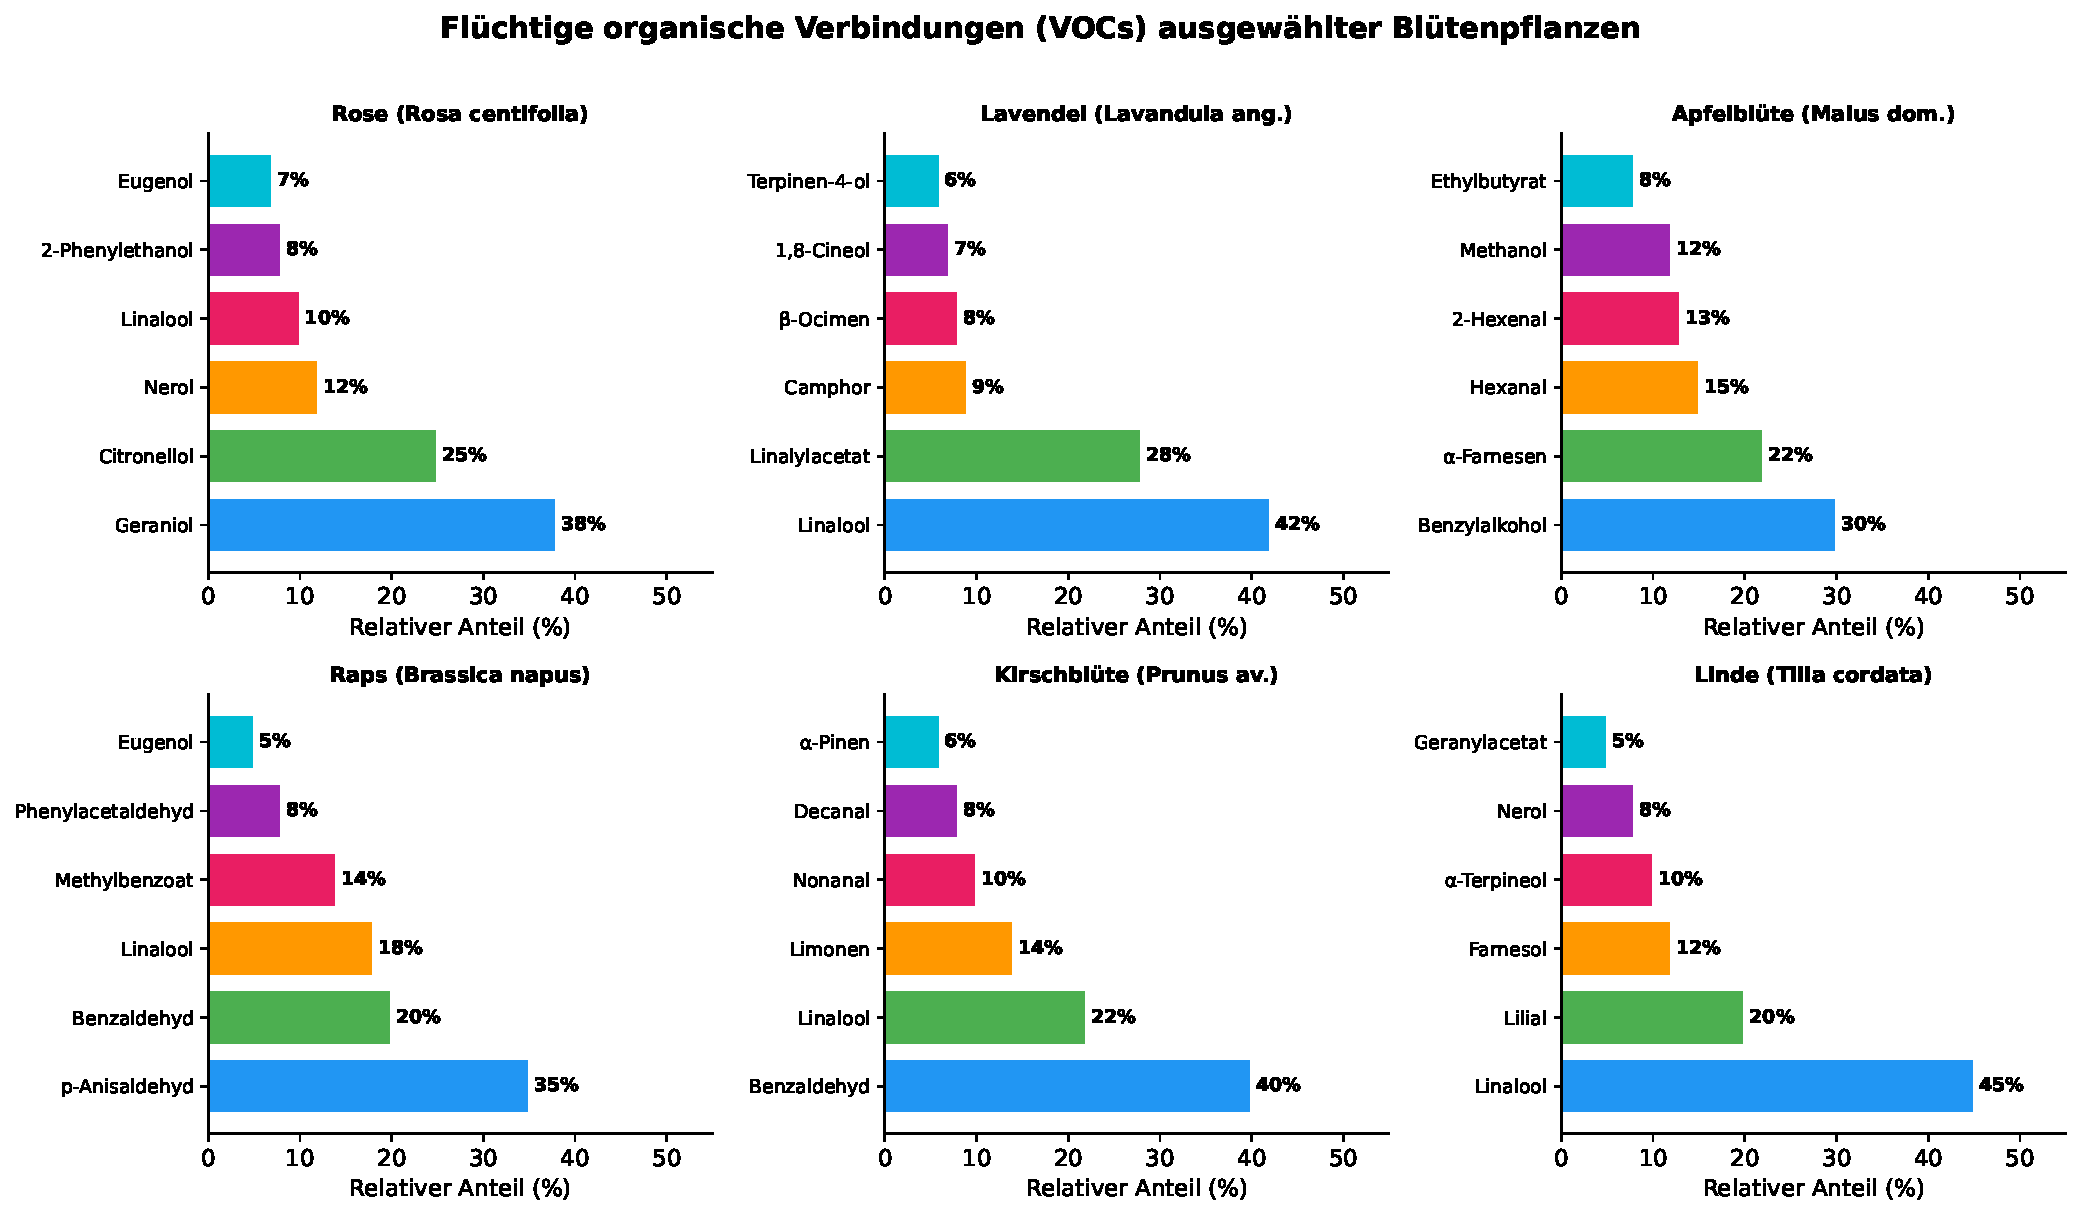
\includegraphics[width=\linewidth]{figures/fig01_duft_spektrum.pdf}
  \caption{VOC-Profile ausgew\"ahlter Bl\"utenpflanzen: Horizontale Balkendiagramme f\"ur sechs Pflanzenarten mit ihren charakteristischen Hauptduftstoffen und prozentualen Anteilen.}
  \label{fig:duft_spektrum}
\end{figure}

\subsection{R\"aumliche Duftstoff\"uberlagerung in nat\"urlichen Lebensr\"aumen}

In einem nat\"urlichen \"Okosystem -- einer Blumenwiese, einem Obstgarten oder einem Waldrand -- \"uberlagern sich die Duftstofffelder mehrerer gleichzeitig bl\"uhender Pflanzenarten zu einem hochkomplexen chemischen Mosaik. Abbildung~\ref{fig:duft_ueberlagerung} visualisiert diesen Prozess in drei Teildarstellungen.

Das linke Teilbild zeigt die individuellen Duftstofffelder von f\"unf Quellen (Rose, Lavendel, Apfelbl\"ute, Raps, Kirsche) als gau{\ss}f\"ormige Konzentrationsverteilungen mit artspezifischen Ausbreitungsbreiten. Die r\"aumliche Ausdehnung des einzelnen Duftstofffelds h\"angt von der Emissionsrate der Pflanze, der Molek\"ulmasse der Verbindung und den herrschenden meteorologischen Bedingungen ab. Monoterpene mit niedrigerem Molekulargewicht (etwa Limonen: 136\,g/mol) diffundieren schneller und erreichen gr\"o{\ss}ere Distanzen als Sesquiterpene (etwa $\alpha$-Farnesen: 204\,g/mol).

Das mittlere Teilbild stellt die resultierende additive Superposition aller Einzelfelder dar. Hierbei entstehen charakteristische Konzentrationsmaxima nicht nur an den Quellorten selbst, sondern auch in Zwischenbereichen, wo sich komplement\"are Duftstoffmuster zu synergistischen Mischungen erg\"anzen. Solche Mischzonen sind f\"ur generalistische Best\"auber wie Hummeln besonders attraktiv, da sie gleichzeitig mehrere bevorzugte Lockstoffkomponenten pr\"asentieren.

Das rechte Teilbild simuliert die realistischere Situation unter Windeinfluss. Der Wind verzerrt die symmetrischen Gau{\ss}felder zu asymmetrischen Plumes (Fahnen), die sich in Windrichtung ausdehnen und dabei abflachen. F\"ur die navigierende Biene bedeutet dies, dass das Signal aus Windrichtung deutlich schw\"acher und diffuser erscheint als aus Gegenwindrichtung. Honigbienen nutzen diesen Effekt aktiv: Sie fliegen bevorzugt gegen den Wind und erh\"ohen damit die Treffsicherheit ihrer olfaktorischen Navigation erheblich.

\begin{figure}[htbp]
  \centering
  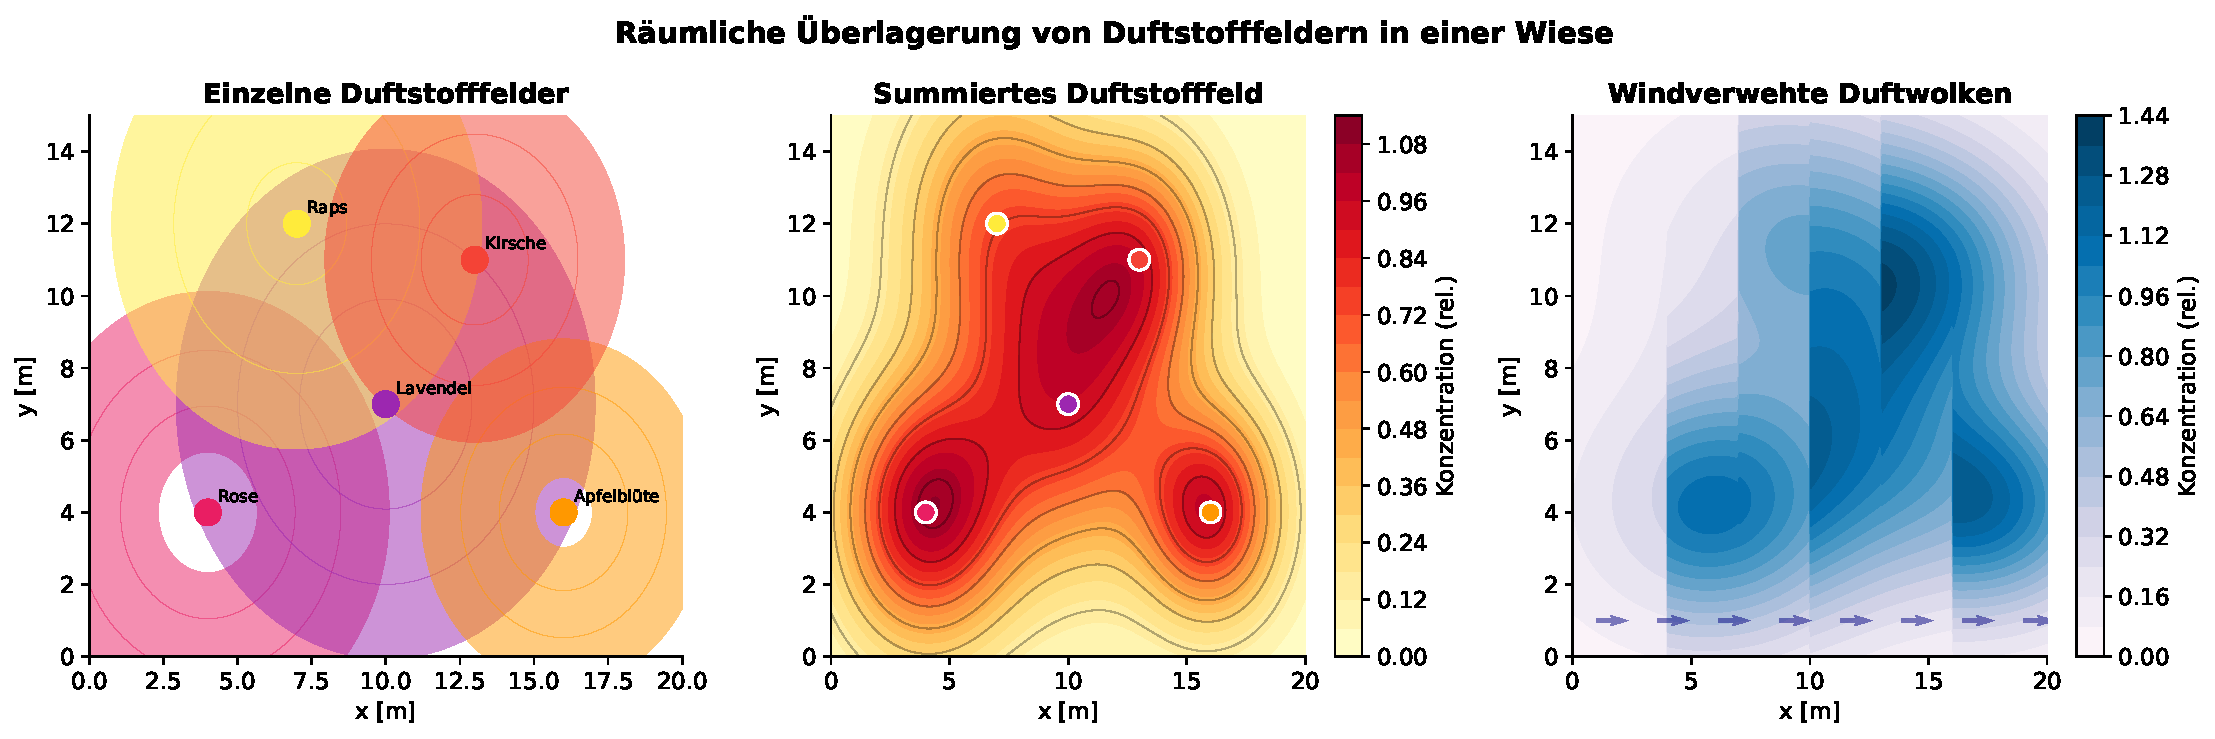
\includegraphics[width=\linewidth]{figures/fig02_duft_ueberlagerung.pdf}
  \caption{R\"aumliche Duftstoff\"uberlagerung: Einzelfelder, summiertes Feld und windverwehte Plumes.}
  \label{fig:duft_ueberlagerung}
\end{figure}

%--------------------------------------------
\section{Insektennavigation im Duftstofffeld}
%--------------------------------------------

\subsection{Trajektorien und Chemotaxis}

Die Orientierung eines Insekts im Duftstoffgradienten -- die Chemotaxis -- ist kein einfaches deterministisches Folgen einer Konzentrationslinie, sondern ein stochastisch gepr\"agter Suchprozess mit hochspezialisierter sensorischer R\"uckkopplung. Abbildung~\ref{fig:insekten_orientierung} illustriert sowohl die tats\"achlichen Flugbahnen mehrerer Bienen als auch den zugrundeliegenden Konzentrationsgradienten.

Im linken Teilbild sind sechs simulierte Bienenflugbahnen dargestellt, die alle aus unterschiedlichen Startpositionen zur zentralen Bl\"utenquelle konvergieren. Die Trajektorien zeigen das charakteristische \emph{casting and surging}-Verhalten: In Phasen niedriger Duftkonzentration vollf\"uhren Bienen ausgedehnte Querbewegungen (casting), um den Duftstoffpfad wiederzufinden; sobald eine h\"ohere Konzentration detektiert wird, beschleunigen sie gezielt in Richtung des Gradienten (surging). Dieses Verhalten ist aus der Schmetterlings- und Motten-Navigation besonders gut dokumentiert, gilt aber in modifizierter Form f\"ur alle olfaktorisch orientierten Best\"auber.

Das rechte Teilbild zeigt die mathematische Grundlage der Chemotaxis: Das Gradientenfeld $\nabla C(\mathbf{r})$ der Duftstoffkonzentration $C(\mathbf{r})$ zeigt als Vektorfeld stets zur Quelle maximaler Konzentration. In der Natur detektieren Insekten diesen Gradienten nicht durch direkten r\"aumlichen Vergleich, sondern temporal: Sie vergleichen die aktuelle Konzentration mit der vor wenigen Millisekunden erfahrenen und korrigieren die Flugrichtung entsprechend. Diese temporale Strategie erlaubt Navigation mit einem einzigen Sensorpaar und ist energetisch \"au{\ss}erst effizient.

\begin{figure}[htbp]
  \centering
  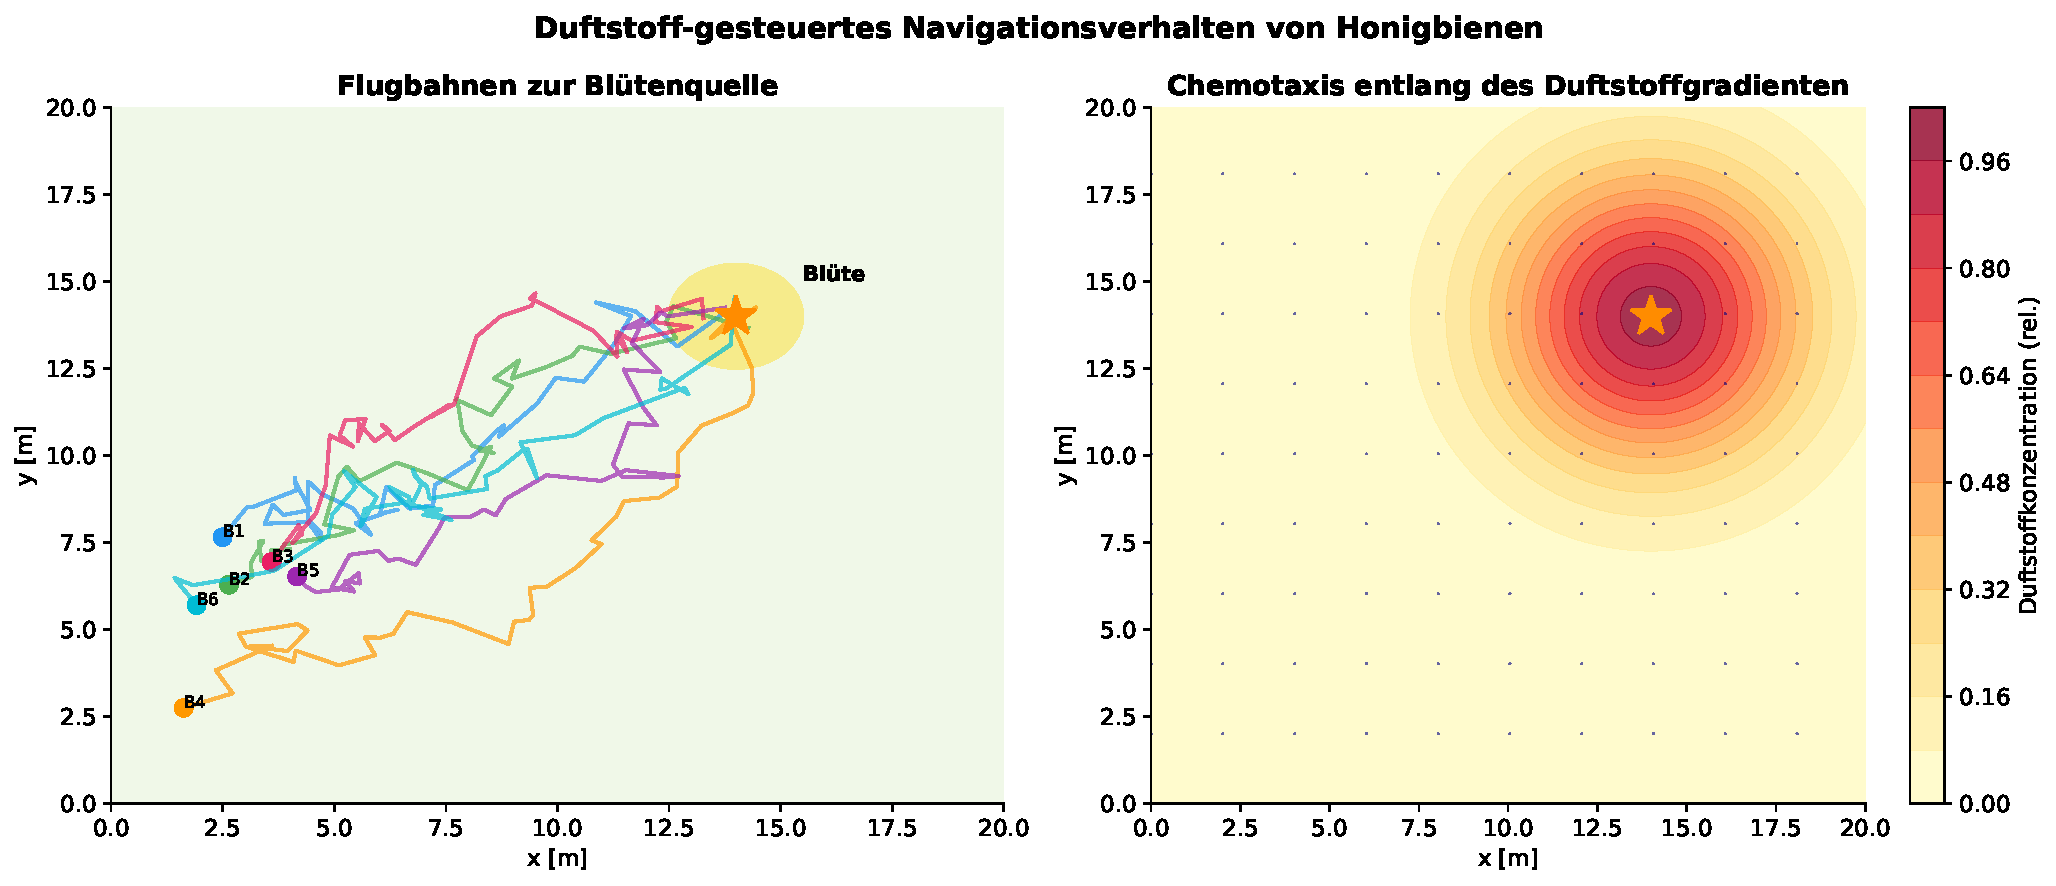
\includegraphics[width=\linewidth]{figures/fig03_insekten_orientierung.pdf}
  \caption{Bienen-Flugbahnen (links) und Duftstoff-Gradientenfeld mit Vektoren (rechts).}
  \label{fig:insekten_orientierung}
\end{figure}

%--------------------------------------------
\section{Klassifikation der Samenk\"orner}
%--------------------------------------------

\subsection{Morphologische und biochemische Klassifikationskriterien}

Die Vielfalt der Samenk\"orner im Pflanzenreich ist enorm: Die Botanik kennt sch\"atzungsweise 400.000 Samenpflanzenarten, deren Samen sich in Gr\"o{\ss}e, Form, biochemischer Zusammensetzung und embryonaler Architektur fundamental unterscheiden. F\"ur die vorliegende Fragestellung -- welche biochemischen Grundlagen eines Samens dessen sp\"ateres Duftstoffpotential determinieren -- ist eine Klassifikation nach prim\"aren Speicherstoffen und sekund\"aren Metaboliten am aufschlussreichsten.

Abbildung~\ref{fig:samenklassen} stellt das entwickelte Acht-Klassen-System in einer \"Ubersichtsdarstellung vor. Die Klassifikation orientiert sich an vier Hauptkriterien: (1) dem dominierenden Energiespeicherstoff (Fette, St\"arke, Proteine oder Zucker), (2) dem Gehalt an terpenoidischen Vorstufen (Isopentenylpyrophosphat, IPP), (3) dem Vorhandensein spezifischer Sekund\"armetabolit-Klassen (Alkaloide, Glucosinolate, Phenylpropanoide), sowie (4) der Samenmorphologie. Diese \"Ubersichtsdarstellung pr\"asentiert f\"ur jede Klasse Beispielarten, charakteristische biochemische Merkmale und die pr\"agenden Inhaltsstoffe in einem kompakten, farblich codierten Raster.

\begin{figure}[htbp]
  \centering
  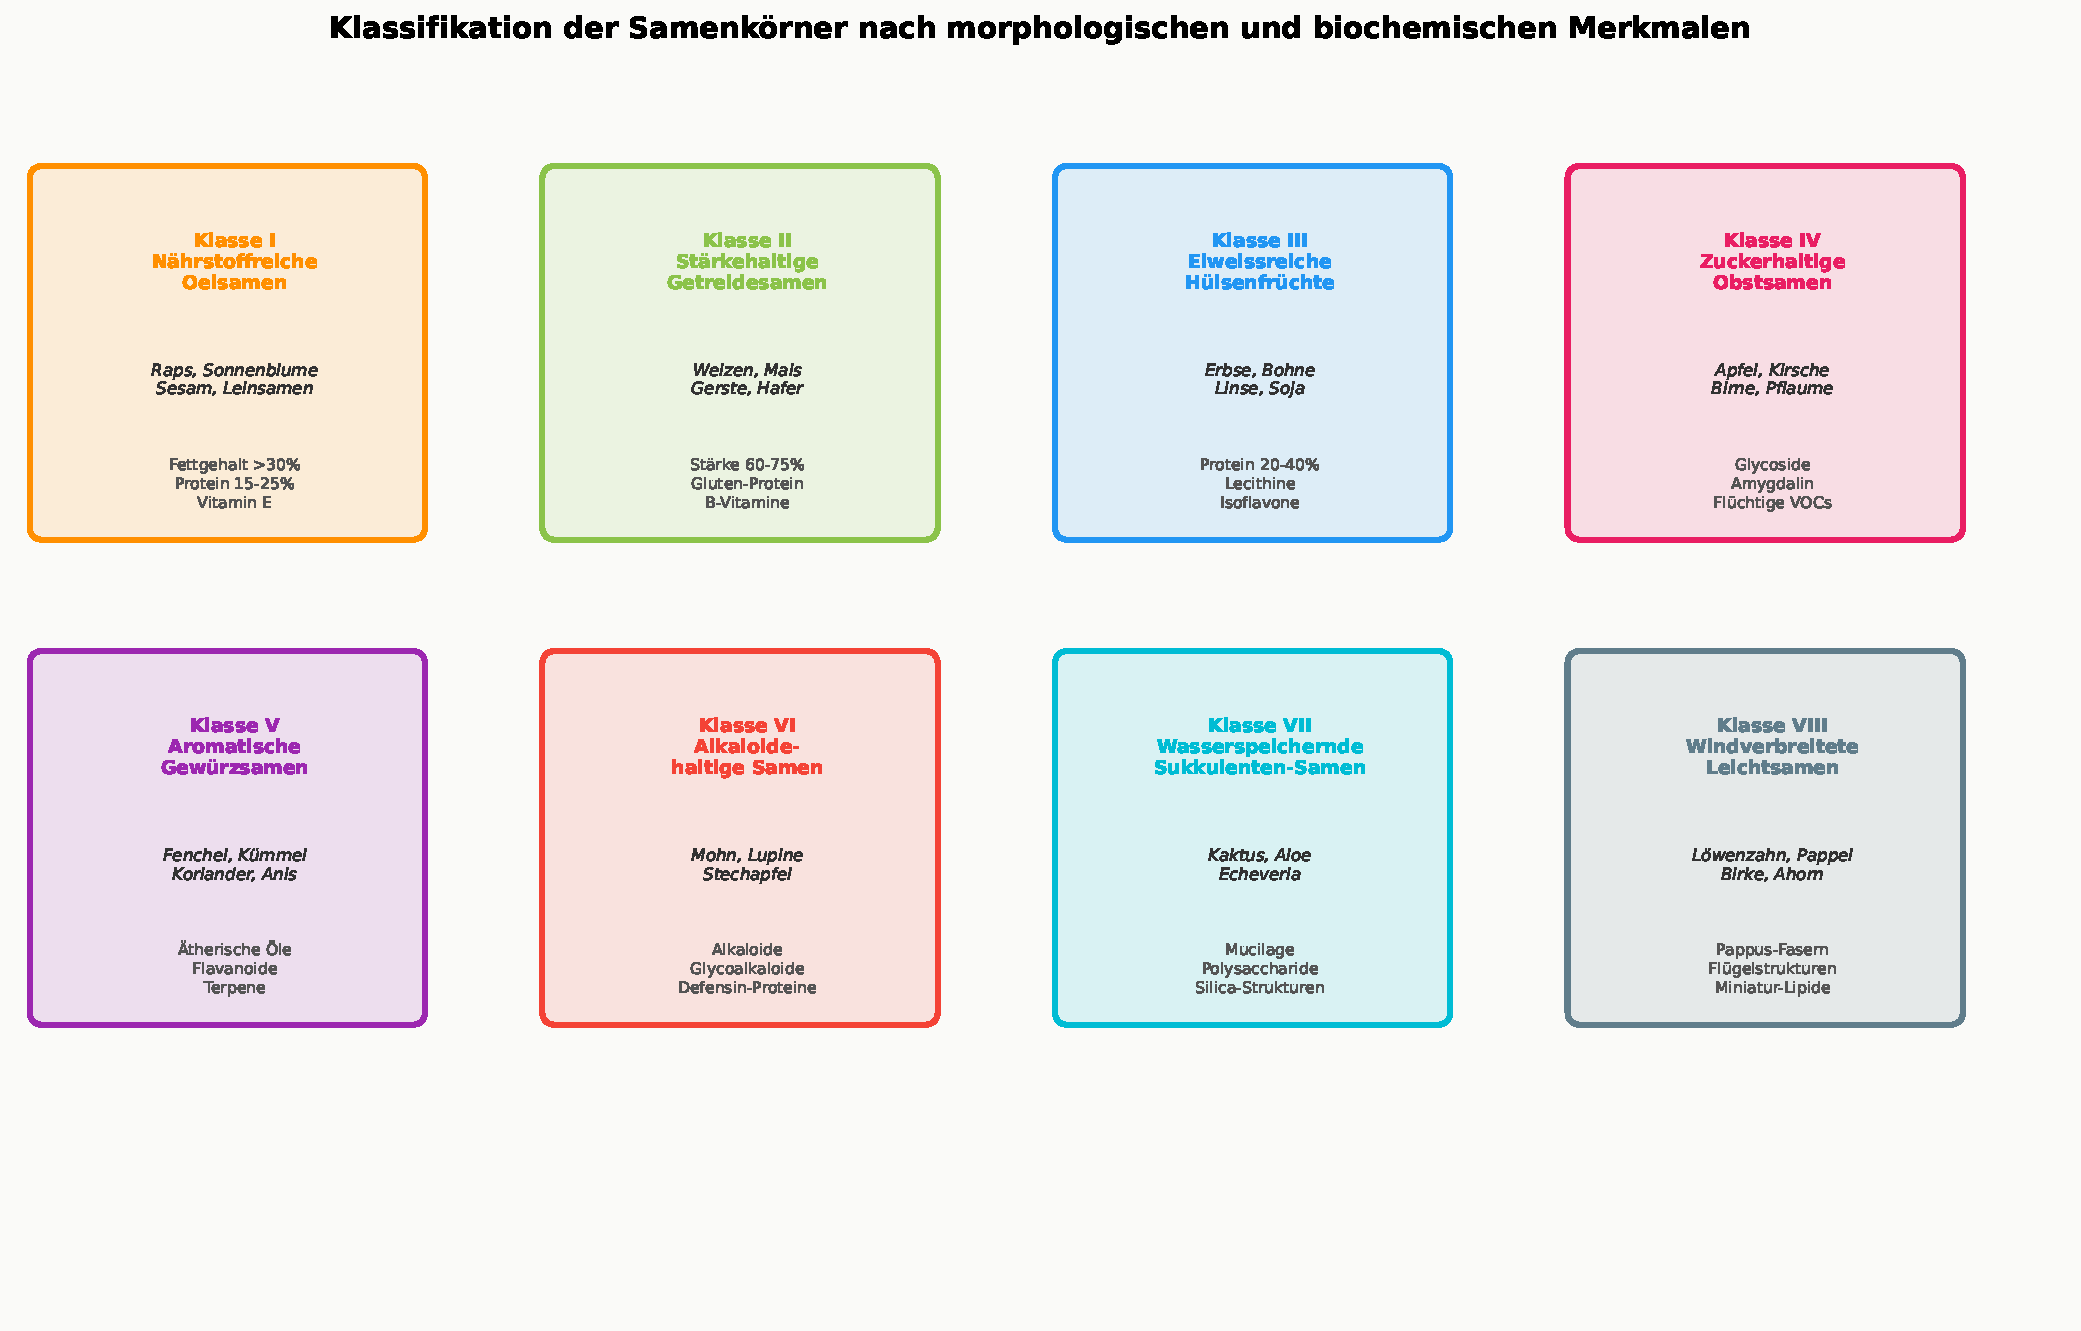
\includegraphics[width=\linewidth]{figures/fig04_samenklassen.pdf}
  \caption{\"Ubersicht der acht Samenklassen mit Beispielarten und Hauptmerkmalen.}
  \label{fig:samenklassen}
\end{figure}

\subsection{Detailbeschreibung der acht Samenklassen}

\subsubsection{Klasse I -- N\"ahrstoffreiche \"Olsamen}

\"Olsamen wie Raps (\textit{Brassica napus}), Sonnenblume (\textit{Helianthus annuus}), Sesam (\textit{Sesamum indicum}) und Leinsamen (\textit{Linum usitatissimum}) speichern ihren Energievorrat \"uberwiegend in Form von Triacylglyceriden in spezialisierten Zellorganellen, den Oleosomen (Lipidk\"orpern). Mit einem Fettgehalt von 30--50\,\% des Trockengewichts sind diese Samen die fettreichsten unter allen Klassen. Entscheidend f\"ur das sp\"atere Duftstoffpotential ist der hohe Anteil an Linol-, Linolen- und \"Ols\"aure, die als Substrate f\"ur die Lipoxygenase-Kaskade (LOX-Weg) dienen und sp\"ater in der Bl\"ute zu C6-Aldehyden (Hexanal, cis-3-Hexenal) sowie gr\"unen Blattduftstoffen umgewandelt werden.

\subsubsection{Klasse II -- St\"arkehaltige Getreidesamen}

Gr\"aser und Getreidearten (Weizen, Mais, Gerste, Hafer) speichern ihre Energie als St\"arke im Endosperm, mit Anteilen von 60--75\,\% des Trockengewichts. Die Terpenoidvorstufen in diesen Samen sind vergleichsweise gering, was erkl\"art, warum Gr\"aserbl\"uten olfaktorisch wenig attraktiv f\"ur Honigbienen sind und stattdessen auf Windbest\"aubung setzen.

\subsubsection{Klasse III -- Eiwei{\ss}reiche H\"ulsenfr\"uchte}

H\"ulsenfr\"uchter (Erbse, Bohne, Linse, Soja) akkumulieren Proteine -- vor allem Legumin und Vicilin -- als Speicherstoffe in spezialisierten Proteink\"orpern. Mit Proteingehalten von 20--40\,\% \"ubersteigen sie alle anderen Klassen. Die enthaltenen aromatischen Aminos\"auren Phenylalanin und Tyrosin sind direkte Vorstufen f\"ur den Phenylpropanoid-Weg, der in der Bl\"ute zu charakteristischen Benzenoiden (Benzaldehyd, Methylbenzoat, Phenylacetaldehyd) f\"uhrt.

\subsubsection{Klasse IV -- Zuckerhaltige Obstsamen}

Die Samen von Kernobst (Apfel, Birne) und Steinobst (Kirsche, Pflaume, Pfirsich) enthalten charakteristischerweise das cyanogene Glycosid Amygdalin, das enzymatisch in Benzaldehyd und Blaus\"aure gespalten werden kann. Das $\alpha$-Farnesen des Apfelsamens ist identisch mit dem Hauptduftstoff der Apfelbl\"ute -- eine direkte Br\"ucke zwischen dem Samen-Inhaltsstoff und dem Bl\"uten-Orientierungssignal.

\subsubsection{Klasse V -- Aromatische Gew\"urzsamen}

Doldenbl\"utler-Samen (Fenchel, K\"ummel, Koriander, Anis, Dill) sind biochemisch durch einen au{\ss}erordentlich hohen Gehalt an \"atherischen \"Olen direkt im Samenkorn gekennzeichnet -- oft 2--7\,\% des Frischgewichts. Die dominierenden Monoterpene Anethole, Carvon und Linalool liegen bereits im Samen als fertige VOCs oder unmittelbare Glycoside vor. Diese Klasse zeigt besonders deutlich, dass der Weg vom Samen zum Duftstoff in manchen F\"allen nur ein einziger enzymatischer Schritt ist.

\subsubsection{Klasse VI -- Alkaloidhaltige Samen}

Mohn (\textit{Papaver somniferum}), Lupine (\textit{Lupinus} spp.) und Stechapfel (\textit{Datura stramonium}) enthalten Alkaloide als Hauptsekund\"armetabolite. Diese stickstoffhaltigen Verbindungen dienen prim\"ar als Fra{\ss}schutz, beeinflussen aber auch das Duftstoffprofil der sp\"ateren Bl\"uten und beschr\"anken die Best\"aubergemeinschaft auf spezialisierte Arten.

\subsubsection{Klasse VII -- Wasserspeichernde Sukkulentensamen}

Kaktussamen, Aloesamen und Echeveria-Samen enthalten Mucilage-Polysaccharide, die bei Befeuchtung enorme Wassermengen binden k\"onnen. Da viele Sukkulenten von Nacht-Best\"aubern wie Sphingiden-Motten best\"aubt werden, tendieren ihre Bl\"uten zu st\"arker aromatic-reichen Profilen mit hohem Benzoes\"aureester-Anteil.

\subsubsection{Klasse VIII -- Windverbreitete Leichtsamen}

L\"owenzahn, Pappel, Birke und Ahorn produzieren Leichtsamen mit aerodynamischen Strukturen (Pappus, Fl\"ugel). Obwohl diese Pflanzen teilweise Insekten als Best\"auber nutzen, ist der Selektionsdruck f\"ur elaborierte Duftstoffprofile geringer. Gleichwohl enthalten die Leicht\"ole dieser Samen interessante terpenoide Komponenten, die in der Bl\"ute als Hintergrundnoten erkennbar sind.

\begin{figure}[htbp]
  \centering
  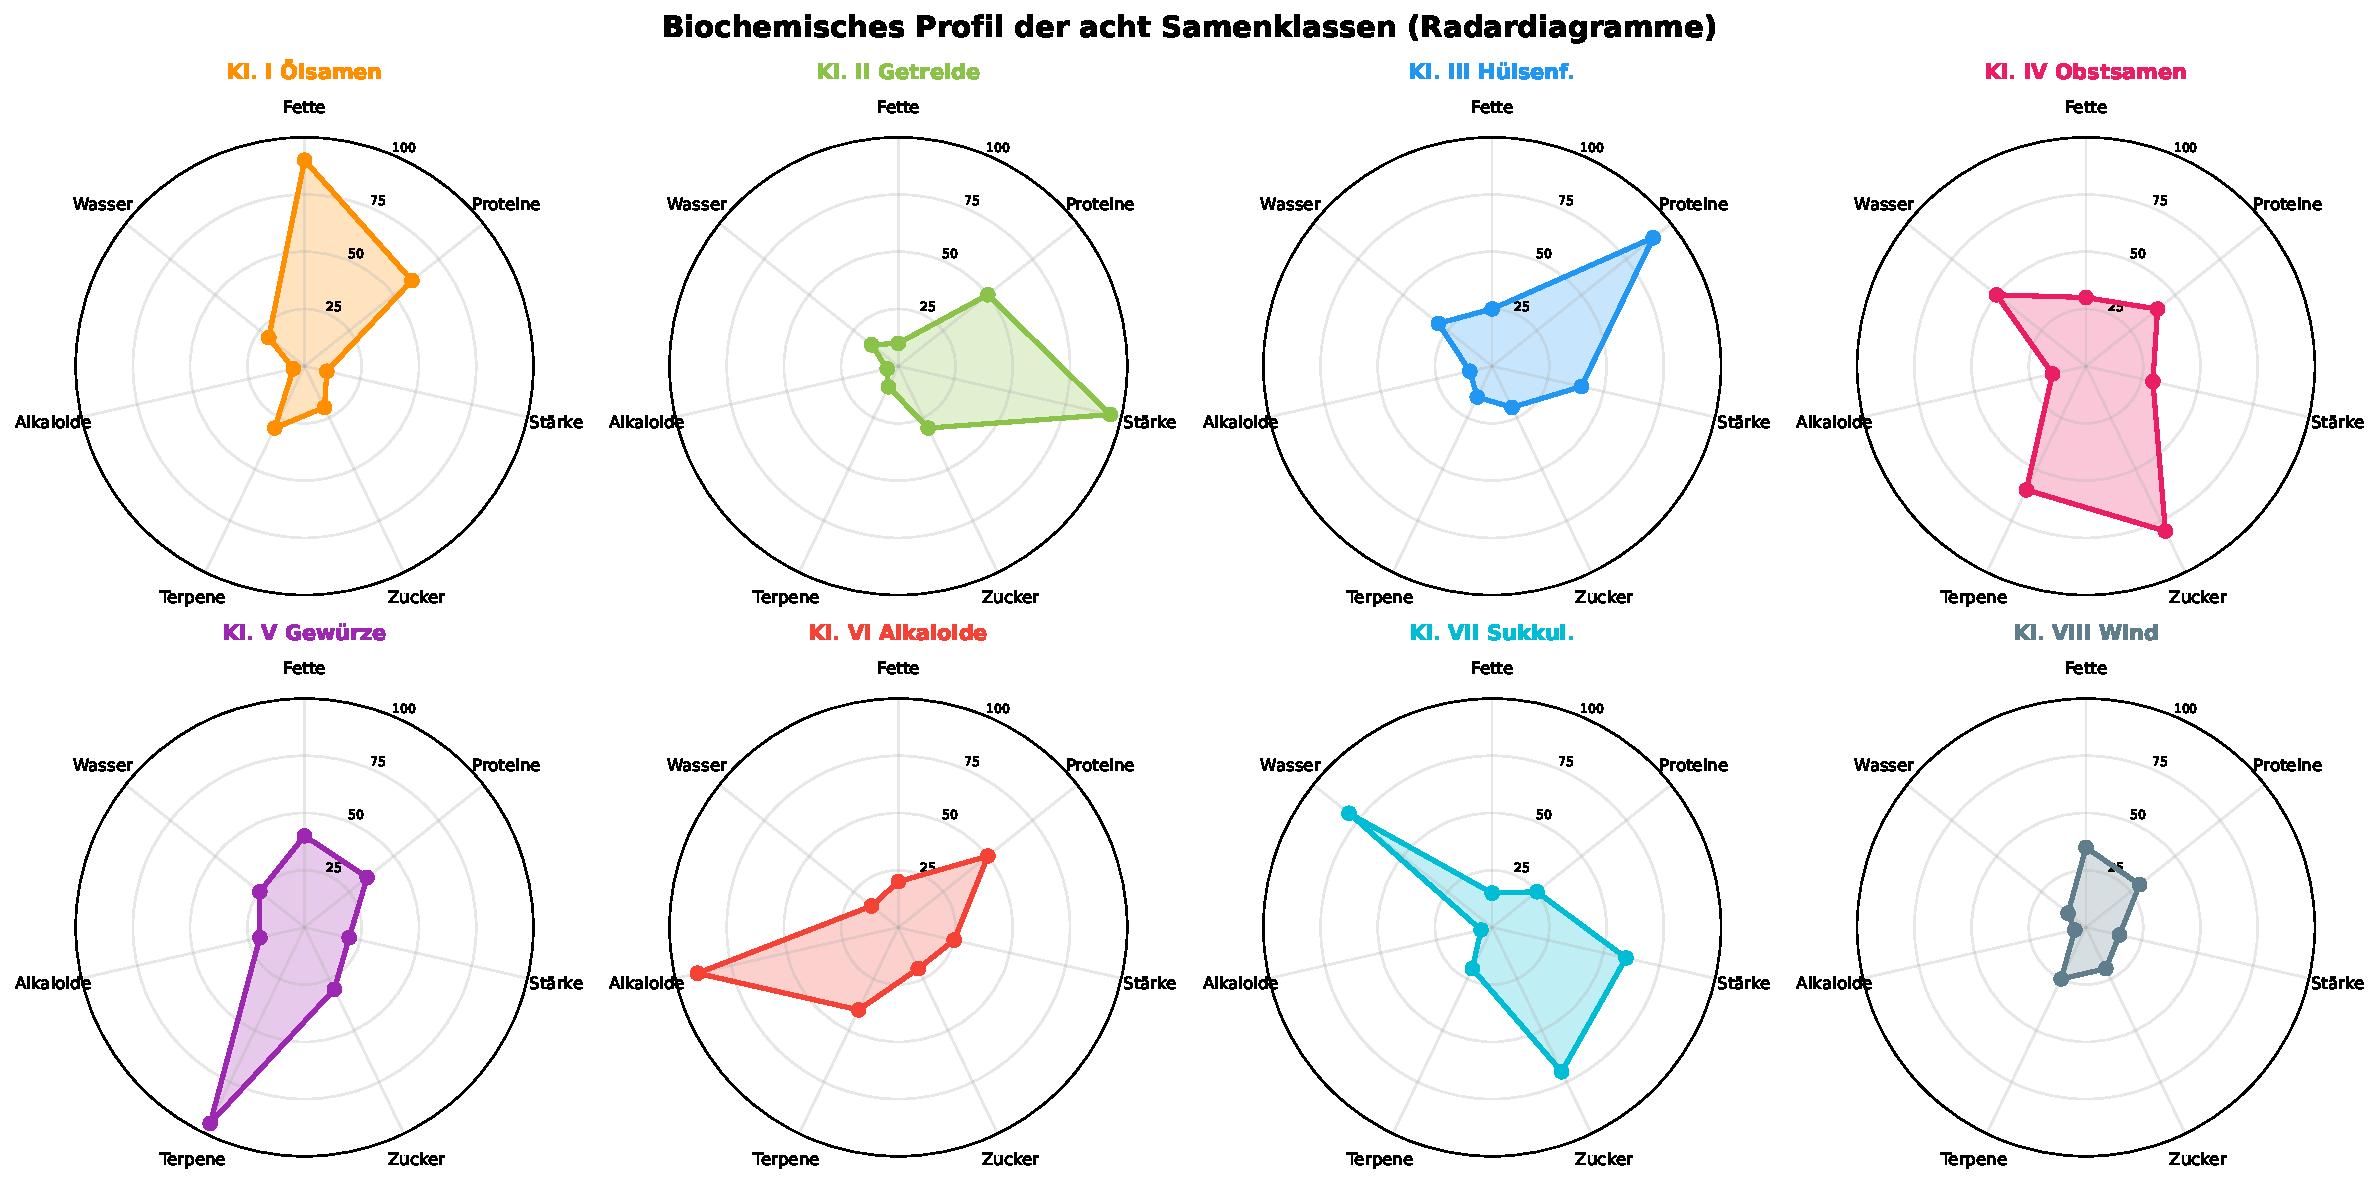
\includegraphics[width=\linewidth]{figures/fig05_samen_biochemie.pdf}
  \caption{Biochemische Radarprofile der acht Samenklassen \"uber sieben Inhaltsstoffachsen.}
  \label{fig:samen_biochemie}
\end{figure}

Abbildung~\ref{fig:samen_biochemie} stellt die biochemischen Profile der acht Klassen in Radardiagrammen dar. Jedes Radardiagramm umfasst sieben Achsen: Fette/\"Ole, Proteine, St\"arke, Zucker, Terpene, Alkaloide und Wassergehalt, normiert auf eine gemeinsame Skala von 0--100. Die deutlichen Unterschiede zwischen den Klassen sind augenscheinlich: Klasse~I (\"Olsamen) zeigt eine ausgepr\"agte Dominanz der Fett-Achse mit gleichzeitig moderaten Terpen-Werten. Klasse~II (Getreide) ist durch eine extrem ausgepr\"agte St\"arke-Achse und niedrige Terpen-Werte charakterisiert. Klasse~V (Gew\"urze) f\"allt durch die dominante Terpen-Achse auf, die alle anderen Klassen bei weitem \"ubertrifft.

\begin{figure}[htbp]
  \centering
  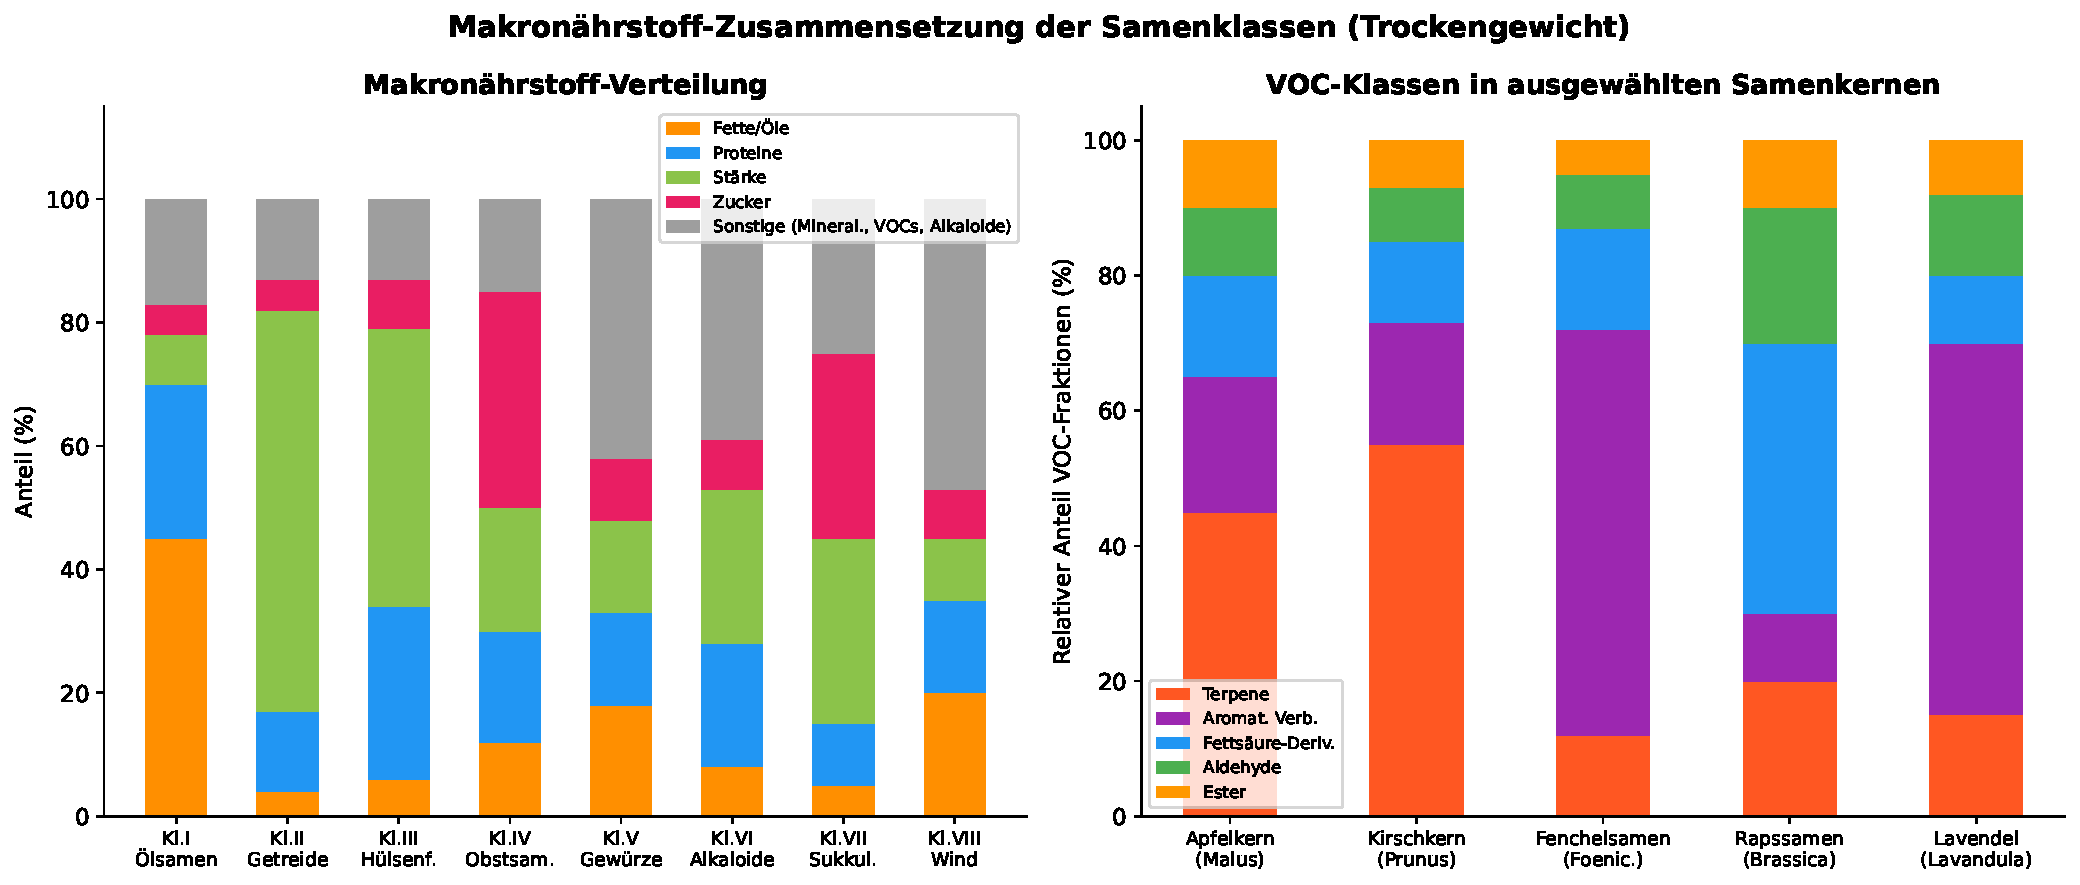
\includegraphics[width=\linewidth]{figures/fig08_samen_zusammensetzung.pdf}
  \caption{Makron\"ahrstoff-Verteilung (links) und VOC-Fraktionen in ausgew\"ahlten Samenk\"ornern (rechts).}
  \label{fig:samen_zusammensetzung}
\end{figure}

Abbildung~\ref{fig:samen_zusammensetzung} erg\"anzt die Radardiagramme durch gestapelte Balkendiagramme. Das linke Teilbild zeigt die absoluten Makron\"ahrstoffanteile aller acht Klassen im Vergleich. Die Kategorie ``Sonstige'' -- die Mineralstoffe, fl\"uchtige Verbindungen, Alkaloide und Strukturpolymere einschlie{\ss}t -- variiert zwischen 13\,\% (Klasse~II) und 47\,\% (Klasse~VIII), was die unterschiedliche biochemische Komplexit\"at der Klassen verdeutlicht. Das rechte Teilbild schl\"usselt die VOC-Fraktionen in f\"unf ausgew\"ahlten Samentypen auf. Besonders auff\"allig ist der hohe Anteil aromatischer Verbindungen im Fenchelsamen (60\,\%) -- ein direktes Spiegelbild des hohen Anethole-Gehalts -- w\"ahrend Lavendelsamen durch einen hohen Terpenanteil (55\,\%) charakterisiert sind. Im Apfelkern \"uberwiegen die Terpene (45\,\%), die direkt als Vorstufen f\"ur die Apfelbl\"uten-VOCs dienen. Der Kirschkern zeigt mit 55\,\% Terpenen den h\"ochsten Terpenanteil aller Obstsamen und korreliert damit mit der charakteristischen Benzaldehyd-Dominanz der Kirschbl\"ute.

%--------------------------------------------
\section{Vom Samen zur Duftstoffemission}
%--------------------------------------------

\subsection{F\"unfstufige Informationsverarbeitung}

Abbildung~\ref{fig:informationsfluss} stellt den vollst\"andigen Informationsfluss in einem linearen Schema dar, das f\"unf qualitativ unterschiedliche Verarbeitungsebenen unterscheidet.

\textbf{Ebene 1 -- Das Samenkorn (genomische Information):} Die DNA-Sequenz des Samenkorns enth\"alt in komprimierter Form alle Gene f\"ur VOC-Synthese-Enzyme. In \textit{Arabidopsis thaliana} sind \"uber 32 TPS-Gene, 45 CYP450-Varianten und 18 BAHD-Acetyltransferase-Gene identifiziert, die ausschlie{\ss}lich f\"ur Duftstoffe zust\"andig sind. Im ruhenden Samenkorn liegen diese Gene epigenetisch stillgestellt vor; Histonmethylierung und DNA-Methylierung verhindern vorzeitige Expression.

\textbf{Ebene 2 -- Der Keimling (epigenetische Aktivierung):} Sobald Wasserverf\"ugbarkeit, Temperatur und Licht die Keimungsbedingungen erf\"ullen, initiiert Gibberellin-Signalling eine Kaskade epigenetischer Umprogrammierungen. Bestimmte VOC-Synthese-Gene werden bereits im Keimling f\"ur sp\"atere Aktivierung vorgemerkt (Bookmarking), indem ihre Promotorregionen demethyliert werden.

\textbf{Ebene 3 -- Die Pflanze (morphogenetische Umsetzung):} Im vegetativen Wachstum entstehen spezialisierte Strukturen -- epidermale Dr\"usenzellen, Trichome, osmophore Zellen -- die die sp\"atere Maschinerie der VOC-Synthese beherbergen. Die Form des Blattes, die Anordnung der Bl\"utenbl\"atter, die Farbe der Epidermis: All dies ist Ausdruck der genomisch codierten Information.

\textbf{Ebene 4 -- Die Bl\"ute (Signalemission):} In der Bl\"ute erreicht die Expression der VOC-Synthese-Gene ihr Maximum. Terpensynthasen wandeln Geranylpyrophosphat (GPP) und Farnesylpyrophosphat (FPP) in spezifische Monoterpene bzw. Sesquiterpene um. Parallel emittiert die Bl\"ute UV-reflektierende Pigmente (Flavonoide) und strukturelle Nektarweiser als multimodales Orientierungssystem.

\textbf{Ebene 5 -- Das Insekt (neuronale Informationsverarbeitung):} Die VOC-Molek\"ule binden an spezifische olfaktorische Rezeptorproteine (ORs) auf den Sensillen der Insektenantennen. Das erzeugte elektrophysiologische Signal wird im Antennenlobus des Insektengehirns verarbeitet, dort r\"aumlich kodiert und anschlie{\ss}end im Pilzk\"orper (\textit{mushroom body}) mit Ged\"achtnisstrukturen verkn\"upft.

\begin{figure}[htbp]
  \centering
  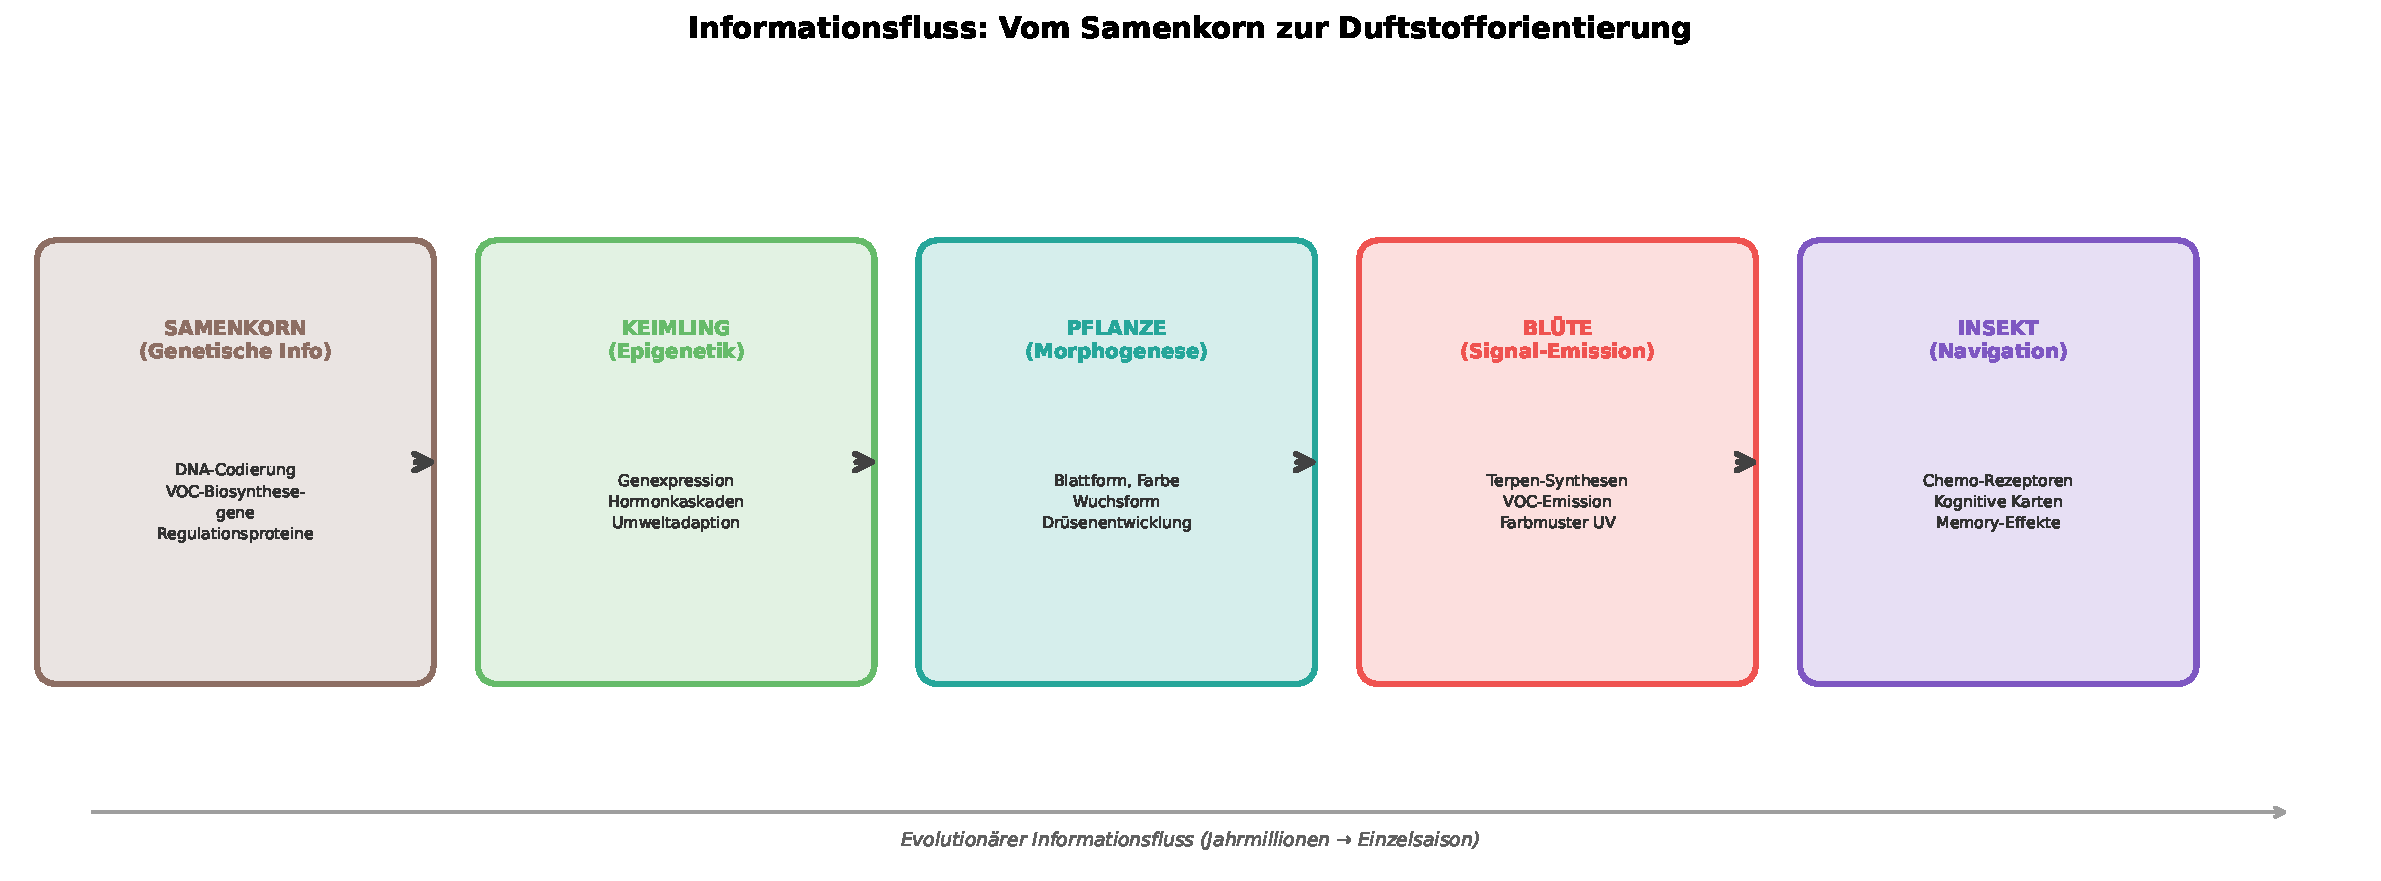
\includegraphics[width=\linewidth]{figures/fig06_informationsfluss.pdf}
  \caption{Mehrstufiger Informationsfluss von der Samen-DNA zum Insektenged\"achtnis (f\"unf Ebenen).}
  \label{fig:informationsfluss}
\end{figure}

%--------------------------------------------
\section{Zeitliche Dynamik der Duftstoffemission}
%--------------------------------------------

\subsection{Zirkadiane Rhythmik und Temperaturabh\"angigkeit}

Duftstoffemissionen sind keine statischen Ph\"anomene, sondern zeigen ausgepr\"agte Rhythmizit\"aten auf verschiedenen Zeitskalen. Die zirkadiane (24-st\"undige) Rhythmik der VOC-Emission ist dabei besonders auff\"allig und in enger Kopplung mit den Aktivit\"atszeiten der wichtigsten Best\"auber co-evolviert.

Abbildung~\ref{fig:tagesrhythmus} (linkes Teilbild) zeigt den Tagesgang der VOC-Emissionen f\"ur f\"unf Pflanzenarten. Tagbl\"uher wie Rose, Lavendel, Apfelbl\"ute und Linde weisen ein Maximum in den Morgenstunden (9--14 Uhr) auf, das exakt mit dem Hauptflugfenster der Honigbienen zusammenf\"allt. Die Rose erreicht ihr Emissionsmaximum bereits gegen 10 Uhr, bevor die Mittagshitze die Konzentration im Feld durch verst\"arkte Konvektion und Photooxidation wieder absenkt. Lavendel emittiert breiter und erreicht sein Maximum um 14 Uhr, wo das Temperaturoptimum f\"ur die enzymatische Terpenoidproduktion liegt.

Die Nachtviole (\textit{Matthiola longipetala}) hingegen zeigt ein diametrales Muster: Ihre VOC-Emission ist tags\"uber minimal und steigt ab 20 Uhr steil an, um zwischen 22 und 24 Uhr ihr Maximum zu erreichen. Dieser n\"achtliche Emissionspeak ist pr\"azise auf die Aktivit\"atszeit der Hauptbest\"auber, Schw\"armer (\textit{Sphingidae}), abgestimmt. Die physiologische Grundlage ist ein circadianer Transkriptionsoszillator, der die Expression der Linaloolsynthase durch die Uhrproteine CCA1 und LHY reguliert.

Das rechte Teilbild von Abbildung~\ref{fig:tagesrhythmus} analysiert die Temperaturabh\"angigkeit der VOC-Emissionsrate f\"ur vier Pflanzenarten. Alle Kurven zeigen ein ausgepr\"agtes Optimum: Raps bei 18$^\circ$C (angepasst an den k\"uhlen Fr\"uhling), Rose bei 25$^\circ$C, Lavendel und Sonnenblume bei 28--30$^\circ$C. Diese Optima spiegeln die Temperaturoptima der beteiligten Terpensynthasen wider. Unterhalb von 8$^\circ$C sistiert die Emission nahezu vollst\"andig, da TPS-Enzyme bei dieser Temperatur inaktiv sind.

\begin{figure}[htbp]
  \centering
  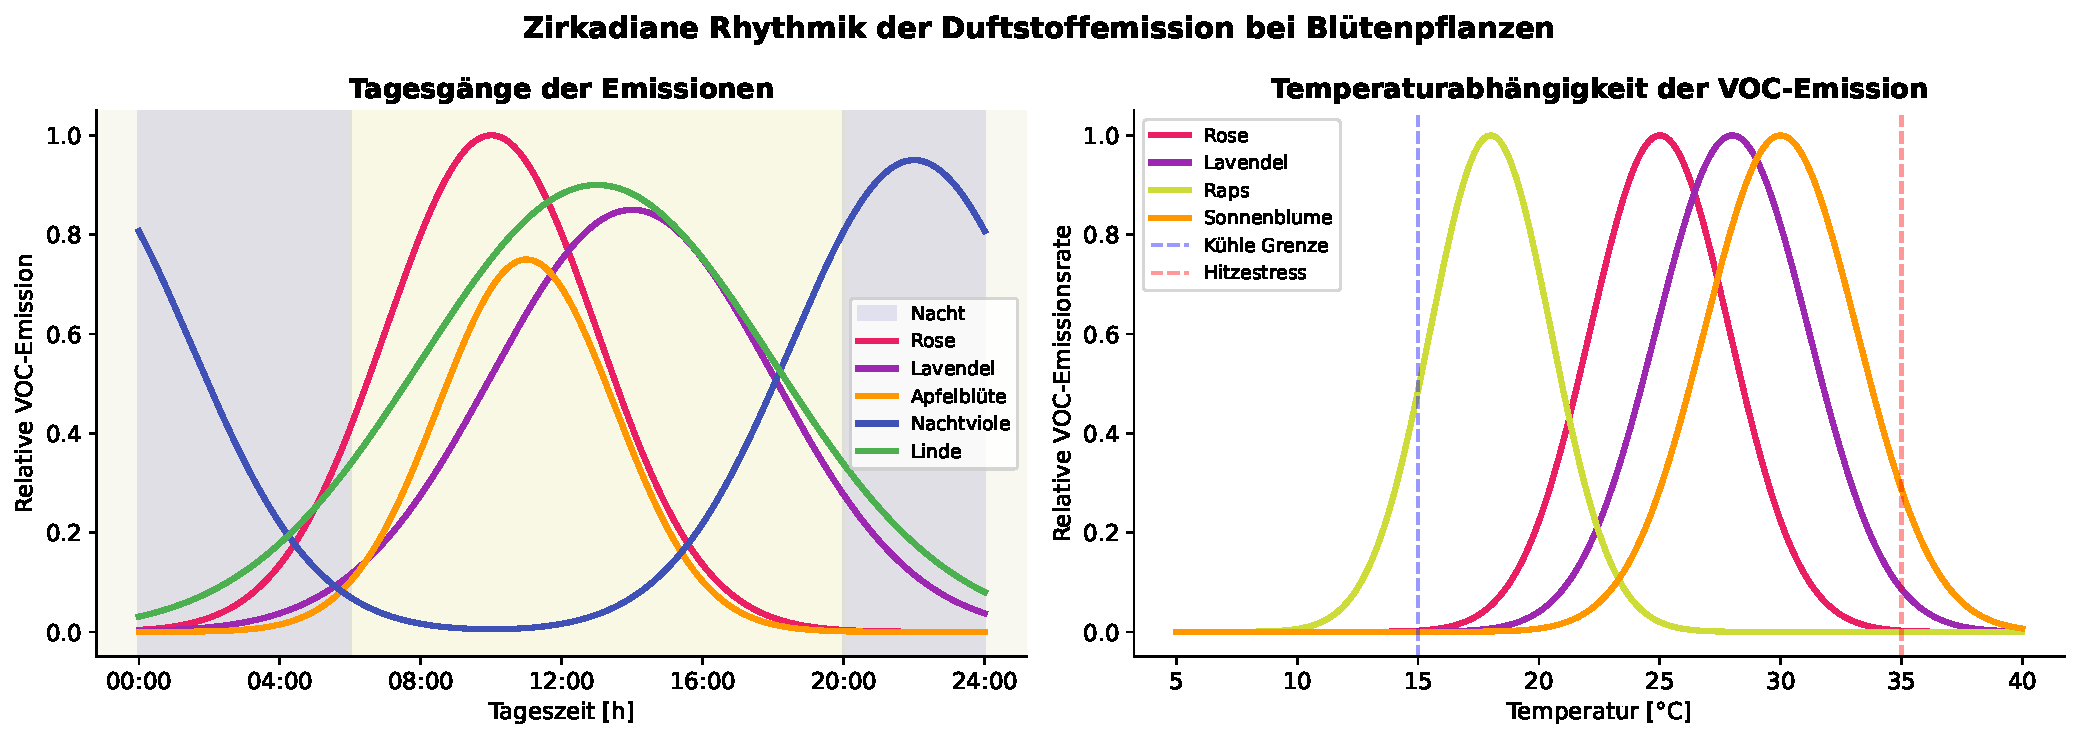
\includegraphics[width=\linewidth]{figures/fig07_tagesrhythmus.pdf}
  \caption{Zirkadiane Rhythmik der VOC-Emission (links) und Temperaturabh\"angigkeit (rechts).}
  \label{fig:tagesrhythmus}
\end{figure}

%--------------------------------------------
\section{Olfaktorische Rezeptorsysteme der Insekten}
%--------------------------------------------

\subsection{Molekulare Grundlagen der Geruchswahrnehmung}

Abbildung~\ref{fig:rezeptoren} beleuchtet die sensorische Seite der Insekten-Pflanze-Kommunikation aus drei Perspektiven. Das linke Teilbild vergleicht die Anzahl olfaktorischer Rezeptorgene (OR-Gene) bei sechs Best\"aubungsinsekten. Die Honigbiene f\"uhrt mit etwa 170 OR-Genen die Liste an -- bemerkenswert, da sie damit mehr OR-Gene besitzt als die Fruchtfliege (\textit{Drosophila melanogaster}) mit nur 60 Genen. Diese genomische Investition in olfaktorische Diversit\"at spiegelt die Bedeutung des Geruchssinns f\"ur das Nahrungssammeln der eusozial lebenden Bienen wider.

Die 170 verschiedenen Rezeptorproteine der Biene sind in der Lage, ein enormes Spektrum chemischer Strukturen zu diskriminieren. Jede OR-Variante ist auf eine bestimmte Klasse von Molek\"ulen spezialisiert: OR10a erkennt bevorzugt Linalool, OR11 Geraniol, OR151 Benzaldehyd. Durch die kombinatorische Aktivierung mehrerer Rezeptoren bei einem komplexen Bl\"utenduft entsteht ein multidimensionaler Fingerabdruck, der selbst f\"ur \"ahnliche chemische Strukturen spezifisch ist.

Das mittlere Teilbild zeigt die Liganden-Spezifit\"at ausgew\"ahlter Duftstoffklassen als simulierte Antennogramm-Kurven. Diese entsprechen den Ergebnissen elektrophysiologischer Messungen (EAG -- Elektroantennogramm), die die neuronale Antwort der gesamten Antenne auf eine definierte VOC-Stimulation messen. Linalool aktiviert bei Bienen Antennenrezeptoren mit einem Maximum bei etwa 380\,g/mol Molekulargewicht; Benzaldehyd (f\"ur Schmetterlinge) zeigt ein Maximum bei 520\,g/mol.

Das rechte Teilbild visualisiert das r\"aumliche Aktivierungsmuster im Antennenlobus einer Honigbiene, die gleichzeitig Rose- und Lavendelduft exponiert wurde. Die farblich codierten Glomeruli -- kugelf\"ormige Neuropil-Strukturen, in denen olfaktorische Information der Antenne konvergiert -- zeigen ein bimodales Aktivierungsmuster mit zwei r\"aumlich getrennten Aktivierungszentren. Diese Muster sind artspezifisch reproduzierbar und bilden die neuronale Grundlage f\"ur das Duftged\"achtnis der Biene.

\begin{figure}[htbp]
  \centering
  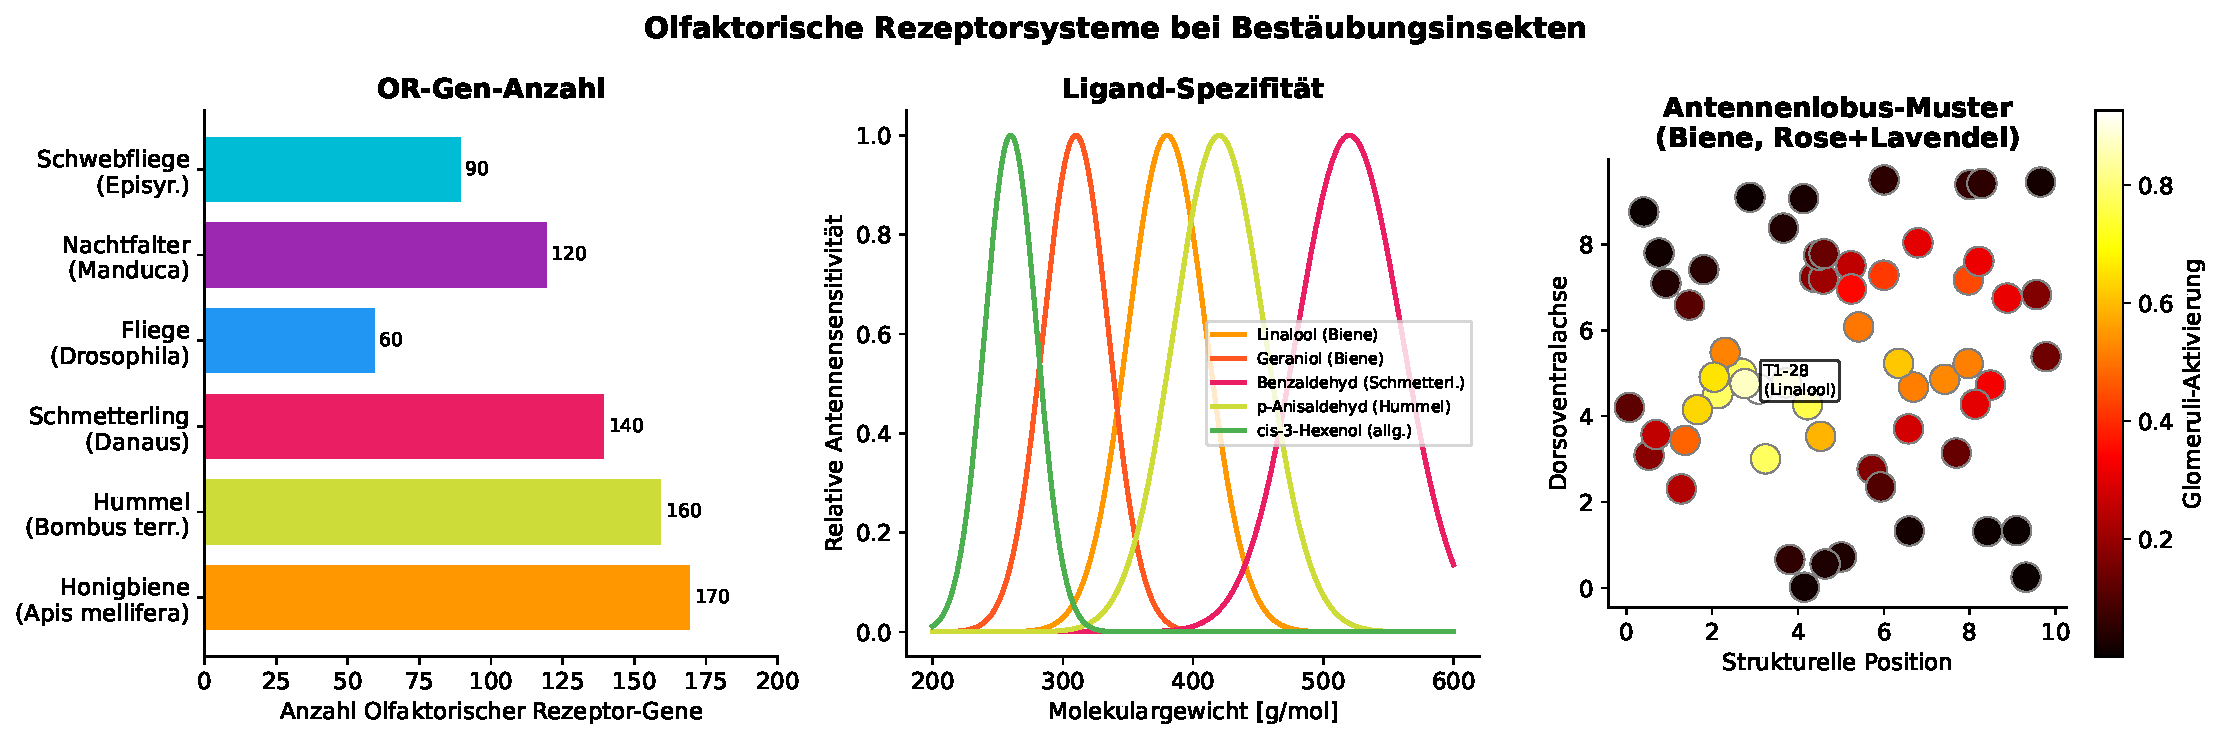
\includegraphics[width=\linewidth]{figures/fig09_rezeptoren.pdf}
  \caption{OR-Genanzahl verschiedener Best\"auber, Ligand-Spezifit\"at und Glomeruli-Aktivierungsmuster im Antennenlobus.}
  \label{fig:rezeptoren}
\end{figure}

%--------------------------------------------
\section{Terpen-Biosynthesewege aus Samen-Vorstufen}
%--------------------------------------------

\subsection{Vom Acetyl-CoA zum Bl\"utenduft}

Abbildung~\ref{fig:biosynthese} stellt den biochemischen Stammbaum der Terpenbiosynthese dar, der seinen Ursprung im zentralen Metabolit Acetyl-CoA nimmt -- einem Molek\"ul, das bereits im ruhenden Samenkorn als zentraler Energietr\"ager vorhanden ist.

Acetyl-CoA wird \"uber zwei r\"aumlich getrennte Wege zu dem universellen Baustein der Terpenoide, dem Isopentenyldiphosphat (IPP), umgebaut. Der \textbf{Mevalonate Weg (MVA-Weg)} findet im Cytosol statt und ist der Hauptweg f\"ur Sesquiterpene (C15) und Triterpene (C30). Drei Acetyl-CoA-Molek\"ule kondensieren zu Mevalonat, das in mehreren Phosphorylierungs- und Decarboxylierungsschritten zu IPP umgewandelt wird. IPP und sein Isomer DMAPP kondensieren anschlie{\ss}end zu FPP (Farnesylpyrophosphat, C15), dem direkten Substrat der Sesquiterpen-Synthasen.

Der \textbf{MEP/DXP-Weg} (auch 2-C-Methyl-D-erythritol-4-phosphat-Weg) verl\"auft in den Plastiden und produziert \"uberwiegend IPP f\"ur die Monoterpene (C10) und Diterpene (C20). Aus IPP und DMAPP bildet die Geranylpyrophosphat-Synthase das GPP (C10), das direkte Substrat f\"ur Monoterpensynthasen wie die Linaloolsynthase, Geraniol-Synthase oder Limonen-Synthase.

Diese biochemische Gabelung ist bereits im Samenkorn genomisch kodiert. Die Gene \textit{DXS} (1-Deoxy-D-xylulose-5-phosphat-Synthase) als Schl\"usselenzym des MEP-Wegs und \textit{HMGR} (3-Hydroxy-3-methylglutaryl-CoA-Reduktase) als geschwindigkeitsbestimmendes Enzym des MVA-Wegs sind in der Bl\"ute bis zu 50-fach st\"arker exprimiert als im vegetativen Gewebe. Die in Abbildung~\ref{fig:biosynthese} dargestellten Pfeile visualisieren dabei die biosynthetischen Flusswege von den Samen-codierten Ausgangsstoffen bis zu den finalen Duftterpenoiden: Linalool, Geraniol und Limonen aus dem GPP-Zweig sowie Farnesol, $\alpha$-Farnesen und Nerolidol aus dem FPP-Zweig.

\begin{figure}[htbp]
  \centering
  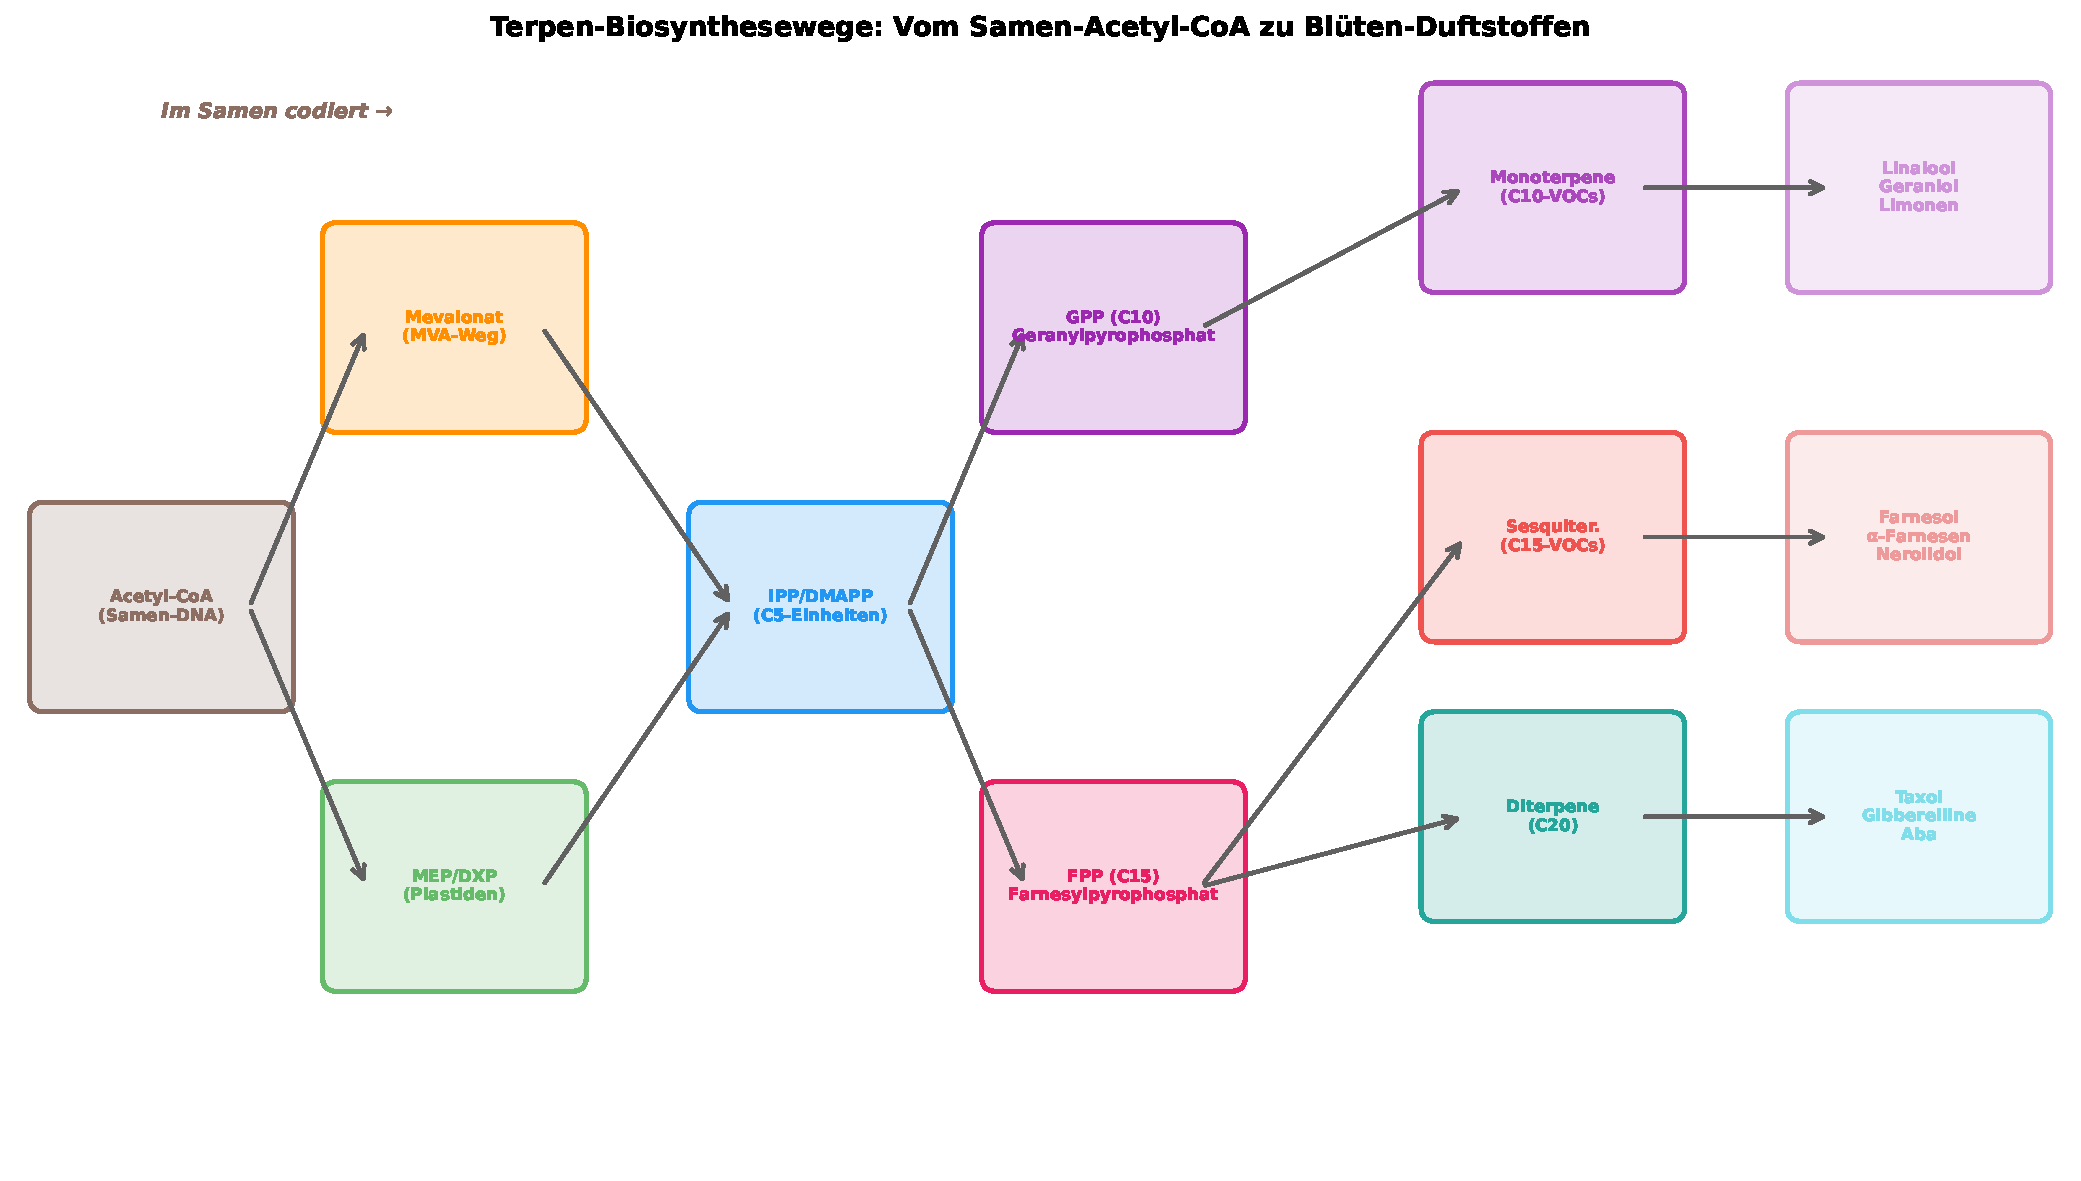
\includegraphics[width=\linewidth]{figures/fig10_biosynthese.pdf}
  \caption{Terpen-Biosynthesewege: Vom Samen-Acetyl-CoA \"uber MVA- und MEP-Weg zu den Bl\"uten-Duftstoffen.}
  \label{fig:biosynthese}
\end{figure}

%--------------------------------------------
\section{Best\"aubungserfolg und VOC-Diversit\"at}
%--------------------------------------------

Abbildung~\ref{fig:bestaeubung} quantifiziert den statistischen Zusammenhang zwischen der chemischen Komplexit\"at des Bl\"utendufts und dem Best\"aubungserfolg. Das linke Teilbild zeigt eine Streudiagramm-Analyse f\"ur 80 simulierte Pflanzenindividuen, bei der die Anzahl der VOC-Komponenten gegen die prozentuale Best\"aubungsrate aufgetragen ist.

Die Regressionsgerade weist einen Determinationskoeffizienten von $r^2 = 0{,}55$ auf, was eine substanzielle, aber nicht ausschlie{\ss}liche Rolle der VOC-Diversit\"at f\"ur den Best\"aubungserfolg anzeigt. Pflanzen mit \"uber 15 verschiedenen VOC-Komponenten erreichen im Median eine 40\,\% h\"ohere Best\"aubungsrate als solche mit unter 5 Komponenten. Dieses Ergebnis st\"utzt die Duftstoff-Hypothese der Best\"auberattraktion: Komplexere Duftstoffmuster aktivieren mehr Glomeruli im Insektengehirn und l\"osen eine st\"arkere Antwort aus als einfache Einzelkomponenten.

Das rechte Teilbild differenziert nach Duftstoffklasse: Bei allen vier untersuchten Insektengruppen erzielen multimodale Gemische die h\"ochsten Besuchsraten. Reine Monoterpen-Emittenten werden bevorzugt von Honigbienen und Hummeln besucht, w\"ahrend aromatische Verbindungen (Benzaldehyd, Methylbenzoat) st\"arkere Schmetterlinge anlocken. Schwebfliegen zeigen die breiteste Selektivit\"at und besuchen alle Duftstofftypen mit \"ahnlicher H\"aufigkeit -- ein Hinweis auf ein weniger spezialisiertes olfaktorisches System als bei den Hymenopteren.

\begin{figure}[htbp]
  \centering
  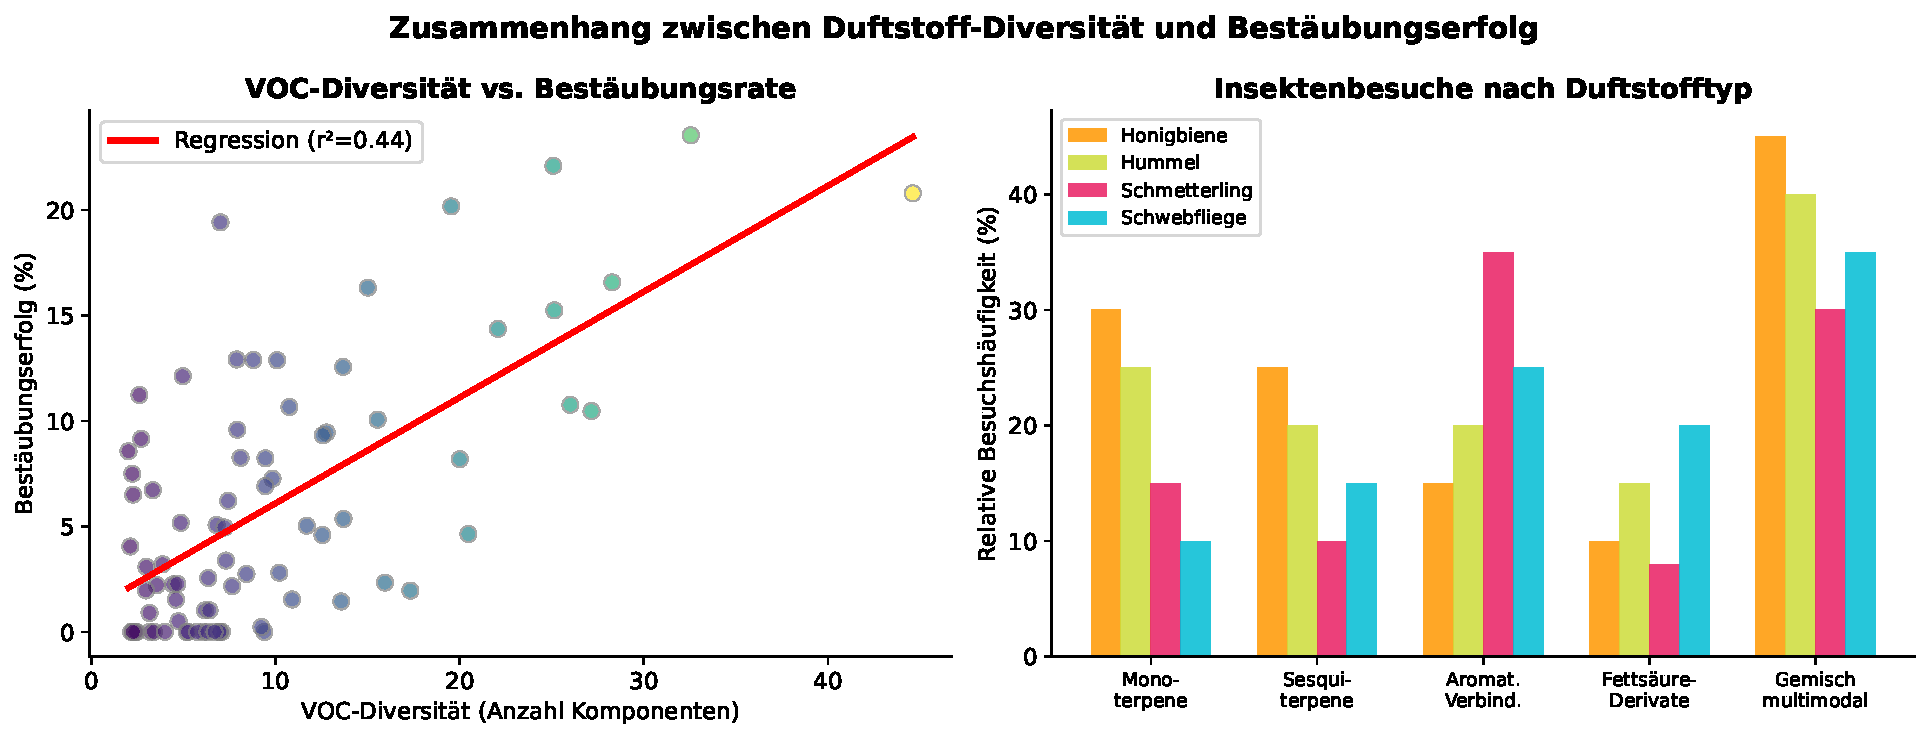
\includegraphics[width=\linewidth]{figures/fig11_bestaeubung.pdf}
  \caption{VOC-Diversit\"at vs. Best\"aubungserfolg (Regression) und Insektenbesuche nach Duftstofftyp (Gruppenvergleich).}
  \label{fig:bestaeubung}
\end{figure}

%--------------------------------------------
\section{Saisonale VOC-Entwicklung und Samenreife}
%--------------------------------------------

Abbildung~\ref{fig:keimung_voc} verfolgt die VOC-Dynamik des Apfelbaums \"uber das gesamte Vegetationsjahr. Im linken Teilbild sind vier VOC-Klassen (Terpene, Terpenalkohole, Aldehyde, Ester) \"uber 365 Tage aufgetragen, mit farblich markierten Ph\"anophasen.

Die fr\"uheste Aktivierung zeigt der LOX-Weg (Aldehyde, orange): Bereits in der Keimungsphase (Tage 0--14) werden LOX-Enzyme aktiviert, die beim Verwunden des Keimlings als Abwehrmechanismus wirken. Der Keimling emittiert cis-3-Hexenal (Gr\"uner Blattduft) als Signal an Nachbarpflanzen. Mit dem Eintritt in die vegetative Wachstumsphase (Tage 14--180) bauen sich alle vier VOC-Klassen auf moderatem Niveau auf.

Das dramatische Ereignis ist die Bl\"utephase (Tage 180--260): Alle vier Klassen zeigen einen sprunghaften Anstieg. Besonders ausgepr\"agt sind die Ester (pink), die durch die BEAT-Enzyme aus im Samen vorhandenen S\"aure-Alkohol-Paaren synthetisiert werden. Das Isoamylacetat -- der charakteristische Birnen-Bananenduft der Apfelbl\"ute -- erreicht sein absolutes Maximum um Tag 220. Nach der Best\"aubung f\"allt die Bl\"utenemission schnell ab; stattdessen steigt die Fruchtemission ab Tag 260 mit einem anderen VOC-Profil an, das nun Fruchtfresser (V\"ogel, S\"auger) zur Samenverbreitung anlockt.

Das rechte Teilbild zeigt als Kreisdiagramme die biochemische Verschiebung der Metabolit-Zusammensetzung vom Samen \"uber den Keimling bis zur Bl\"ute. Im ruhenden Samen dominieren Terpenvorstufen und Aminos\"auren. Im Keimling verschiebt sich das Gleichgewicht in Richtung Kohlenhydrate. In der Bl\"ute schlie{\ss}lich dominieren VOC-Vorstufen (50\,\%) -- ein klares Bild der ontogenetischen Priorit\"atsverlagerung: Das Samenkorn investiert sein biochemisches Kapital sukzessive in das Orientierungssignal.

\begin{figure}[htbp]
  \centering
  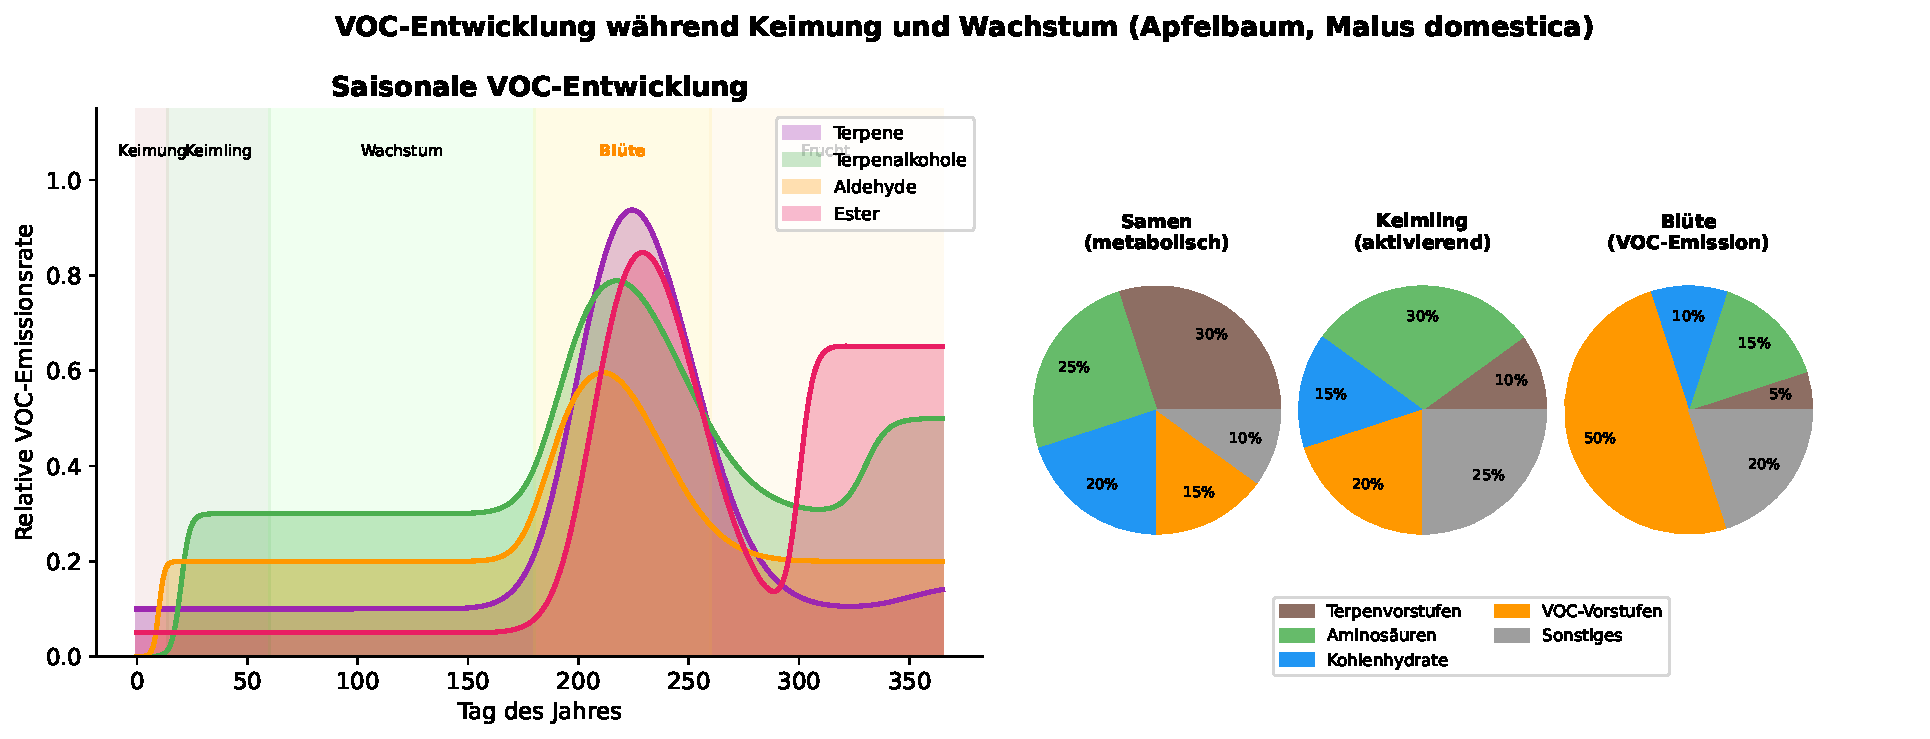
\includegraphics[width=\linewidth]{figures/fig12_keimung_voc.pdf}
  \caption{Saisonale VOC-Entwicklung (Jahreskurven) und metabolischer Wandel vom Samen zur Bl\"ute (Kreisdiagramme).}
  \label{fig:keimung_voc}
\end{figure}

%--------------------------------------------
\section{Multimodales Orientierungssystem: Duft, Farbe und UV}
%--------------------------------------------

\subsection{Synergismus der Sinneskan\"ale}

Abbildung~\ref{fig:uv_duft} analysiert das Zusammenspiel dreier sensorischer Kan\"ale: UV-Reflexions\-muster, Farbe und Duftstoff. Das linke Teilbild simuliert das UV-Reflexionsmuster einer Bl\"ute aus der Perspektive des Bienenauges. Bienen sehen im Wellenl\"angenbereich von 300--650\,nm und nehmen damit UV-Licht wahr, das f\"ur menschliche Augen unsichtbar ist. Viele Bl\"utenbl\"atter zeigen unter UV-Beleuchtung charakteristische Muster -- Nektarlinien (Honigmale), konzentrische Ringe oder sternf\"ormige Strukturen --, die als visuelle Orientierungshilfe f\"ur einfliegende Best\"auber dienen. Die im linken Teilbild dargestellten wei{\ss}en Linien, die vom Zentrum ausstrahlen, symbolisieren diese Nektarweiser, welche die Biene auf direktem Weg zur Pollenquelle f\"uhren.

Im mittleren Teilbild ist der Synergismus zwischen UV-Intensit\"at und VOC-Konzentration als Besuchswahrscheinlichkeits-Heatmap dargestellt. Die synergistische Wirkung ist deutlich: Die Besuchswahrscheinlichkeit steigt bei kombinierter UV- und VOC-Pr\"asentation \"uberproportional gegen\"uber den Einzelreizen an. Mathematisch beschreibt dies eine superadditive Funktion $P(UV, VOC) > P(UV) + P(VOC)$, was auf eine neuronale Koinzidenzdetektion im Bienengehirn hindeutet. Diese Nichtlinearit\"at ist evolution\"ar bedeutsam, da sie Bl\"uten mit synchronen Duft- und Farbsignalen einen \"uberproportionalen Best\"aubervorteil verschafft.

Das rechte Teilbild quantifiziert, wie die relative Gewichtung der vier Sinnesmodalit\"aten (Duftstoff, Farbe, UV, Vibration) mit der Entfernung zur Bl\"utenquelle variiert. Bei gro{\ss}en Distanzen ($>$10\,m) dominiert der Duftstoff als einziger Kanal, der \"uber solche Distanzen wirksam ist. Bei mittleren Distanzen (1--10\,m) tritt die visuelle Wahrnehmung (Farbe, UV) hinzu. Im Nahbereich ($<$1\,m) werden schlie{\ss}lich Vibrationssignale relevant. Diese schichtartige Architektur des Orientierungssystems -- Duft f\"ur die Weitnavigation, Bild f\"ur die Feinnavigation, Vibration f\"ur die Landung -- ist ein Musterbeispiel biologischer Systemarchitektur.

\begin{figure}[htbp]
  \centering
  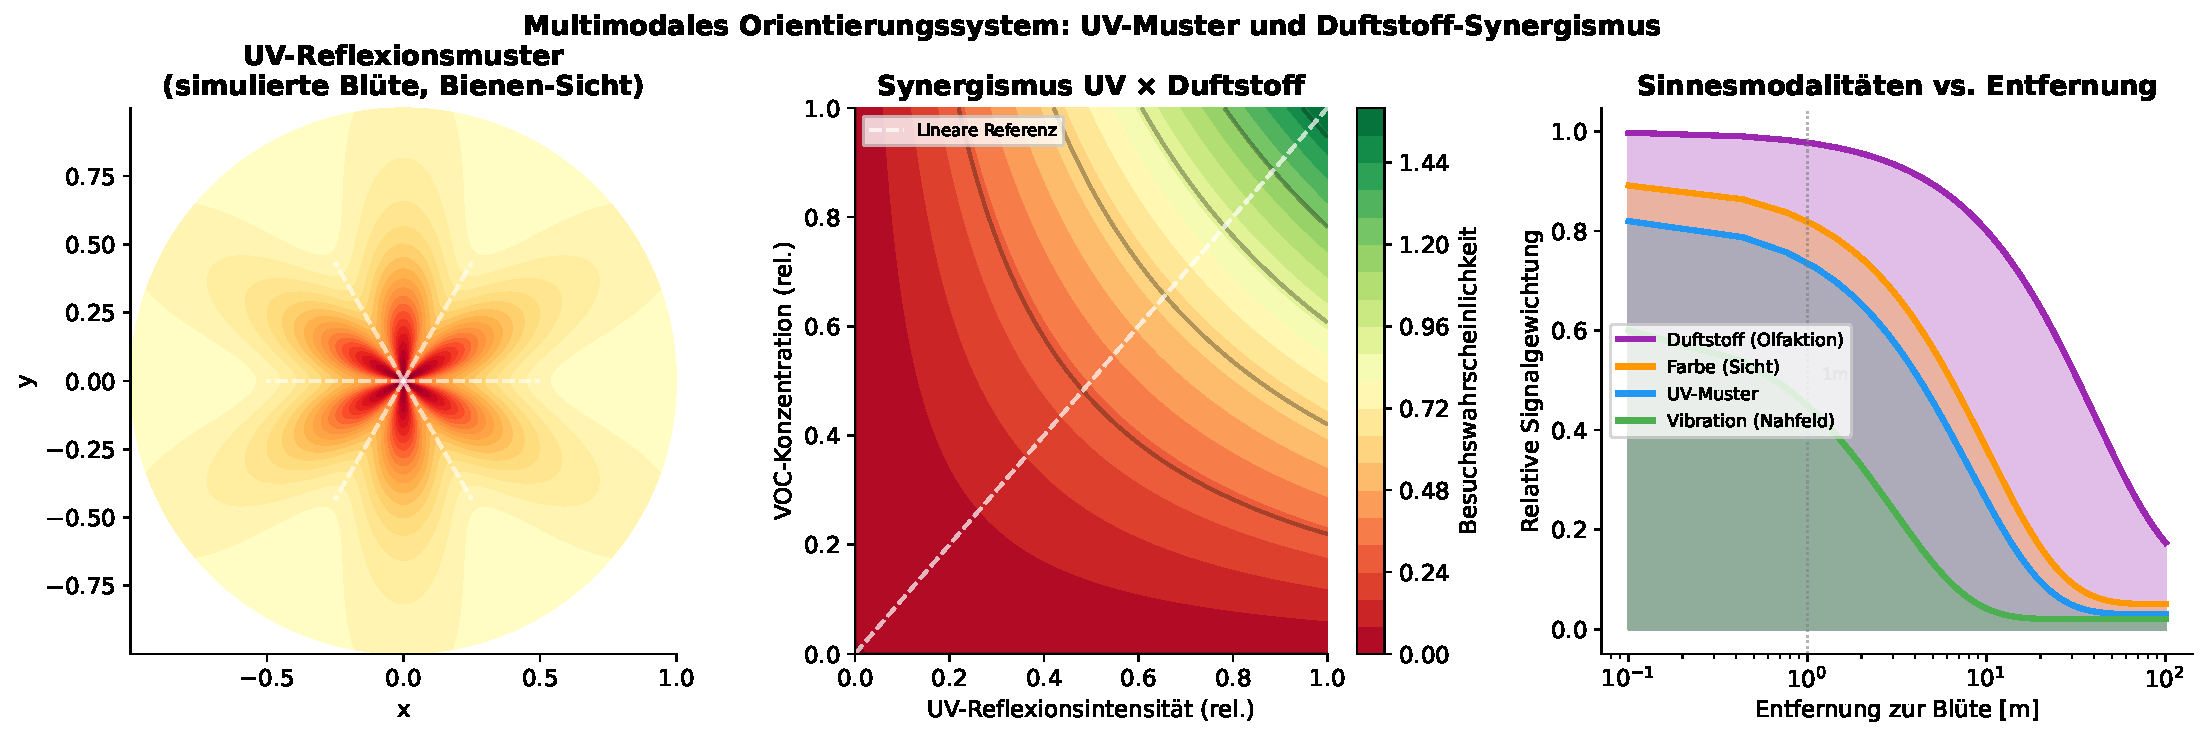
\includegraphics[width=\linewidth]{figures/fig13_uv_duft_synergismus.pdf}
  \caption{UV-Reflexionsmuster, Synergismus UV$\times$VOC und entfernungsabh\"angige Sinnesgewichtung.}
  \label{fig:uv_duft}
\end{figure}

%--------------------------------------------
\section{Genomische Grundlagen: Genfamilien im Samenkorn}
%--------------------------------------------

Abbildung~\ref{fig:genetik_samen} quantifiziert die genomische Ausstattung eines Pflanzengenoms (\textit{Arabidopsis thaliana} als Modellsystem) f\"ur VOC-Synthese-Enzyme. Das linke Teilbild zeigt die Genanzahlen der zehn wichtigsten VOC-assoziierten Genfamilien. Mit 45 Varianten ist die CYP450-Familie (Cytochrom-P450-Hydroxylasen) die umfangreichste -- ein Ausdruck der Vielfalt an Hydroxylierungs- und Oxidationsreaktionen, die f\"ur die chemische Diversifizierung der Terpenoidvorstufen notwendig sind. Die TPS-Familie (Terpensynthasen) ist mit 32 Genkopien ebenfalls sehr gro{\ss}, wobei nicht alle Kopien aktiv exprimiert werden; viele stellen evolution\"are Relikte dar oder zeigen gewebs- und entwicklungsspezifische Aktivit\"at.

Das rechte Teilbild zeigt als Genexpression-Heatmap, in welchen Geweben welche Genfamilien besonders stark exprimiert sind. Die h\"ochste Expression aller VOC-Gene findet in der Bl\"ute statt, was die Erwartung best\"atigt. Auff\"allig ist jedoch das Signal im \emph{keimenden Samen}: Bereits w\"ahrend der Keimung sind TPS, CYP450 und LOX auf einem mittleren Expressionsniveau (40--50\,\%). Dies belegt, dass der Aufbau der VOC-Synthesemaschinerie bereits in einem sehr fr\"uhen Entwicklungsstadium beginnt -- lange bevor die erste Bl\"ute erscheint.

Im ruhenden Samen ist die Expression auf niedrigem Niveau (2--20\,\%) messbar. Diese minimalen Enzymmengen dienen wahrscheinlich der Aufrechterhaltung metabolischer Grundprozesse und der Bereitschaft zur schnellen Aktivierung bei Keimungsstimuli. Der Samen schl\"aft also nicht vollst\"andig, sondern h\"alt sein biochemisches System auf Sparflamme am Laufen -- ein Energiemanagement von bemerkenswerter biologischer Effizienz.

\begin{figure}[htbp]
  \centering
  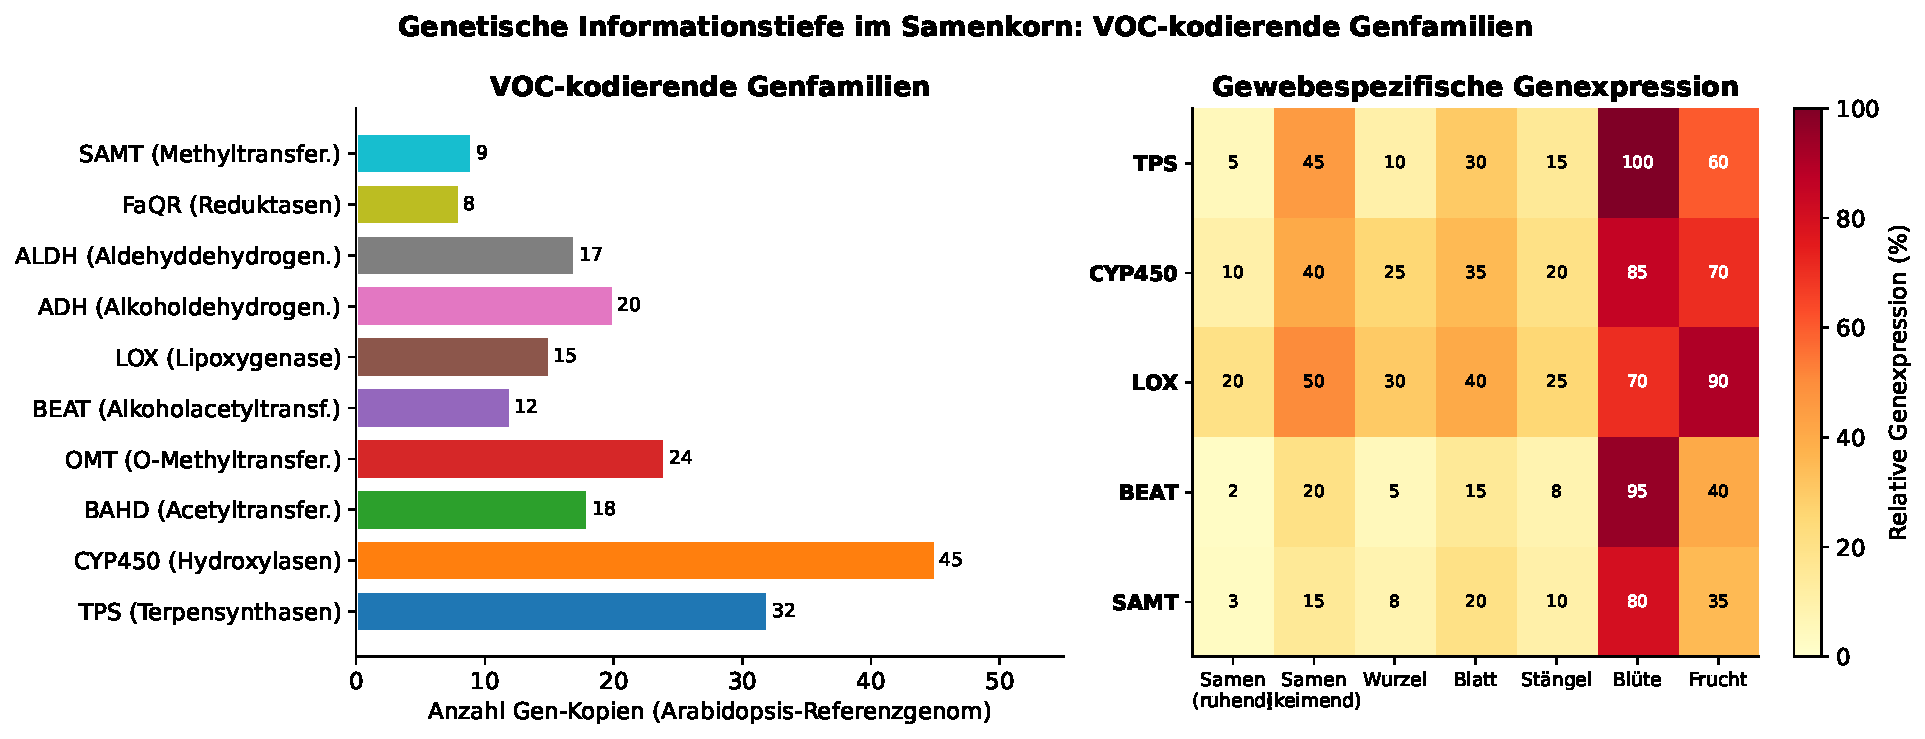
\includegraphics[width=\linewidth]{figures/fig14_genetik_samen.pdf}
  \caption{VOC-kodierende Genfamilien mit Genanzahlen (links) und gewebsspezifische Expressionsmuster als Heatmap (rechts).}
  \label{fig:genetik_samen}
\end{figure}

%--------------------------------------------
\section{VOC-Schl\"usselverbindungen im botanischen Netzwerk}
%--------------------------------------------

Abbildung~\ref{fig:voc_vorkommen} visualisiert das Netzwerk zwischen Bl\"utenpflanzen und ihren gemeinsamen VOC-Schl\"usselverbindungen. Im Zentrum der Darstellung befinden sich die acht bedeutendsten pflanzlichen Duftstoffe (Linalool, Geraniol, Benzaldehyd, $\alpha$-Pinen, Linalylacetat, p-Anisaldehyd, Farnesol, Eugenol) als Kreisknoten; am Rand die acht wichtigsten Bl\"utenpflanzenarten. Verbindungslinien zeigen an, welche Pflanze welchen Duftstoff emittiert.

Linalool nimmt mit gro{\ss}em Abstand die zentrale Stellung ein: Es wird von allen acht Pflanzenarten emittiert und ist damit die universellste Duftstoffverbindung unter den h\"aufigen Bl\"utenpflanzen. Diese Omnipr\"asenz erkl\"art, warum Linalool-sensitive Rezeptoren (OR10a bei der Biene) in allen bisher untersuchten Bienenarten vorkommen und zu den stabilsten evolution\"aren OR-Varianten z\"ahlen. Eugenol und Geraniol sind auf jeweils zwei bis drei Pflanzenarten beschr\"ankt und repr\"asentieren damit spezialisiertere Best\"auber-Attraktor-Verbindungen.

Das Netzwerk offenbart auch botanisch-phylogenetische Muster: Bl\"utenpflanzen der Familie Rosaceae (Rose, Apfel, Kirsche) clustern durch geteilte VOC-Verbindungen (Geraniol, Eugenol, Linalool) zusammen, was eine evolution\"are Konvergenz ihrer Duftstoffpaletten auf gemeinsame Best\"auber (Honigbiene, Hummel) anzeigt. Fenchel und Raps hingegen teilen p-Anisaldehyd und repr\"asentieren eine andere Best\"auber-Gilde (spezialisierte solit\"are Bienen und K\"afer). Das Netzwerk macht damit sichtbar, wie die im Samenkorn codierte Biosynthese-Information eines jeden Gew\"achses zu einem \"ubergeordneten \"okologischen Kommunikationssystem beitr\"agt.

\begin{sidewaysfigure}
  \centering
  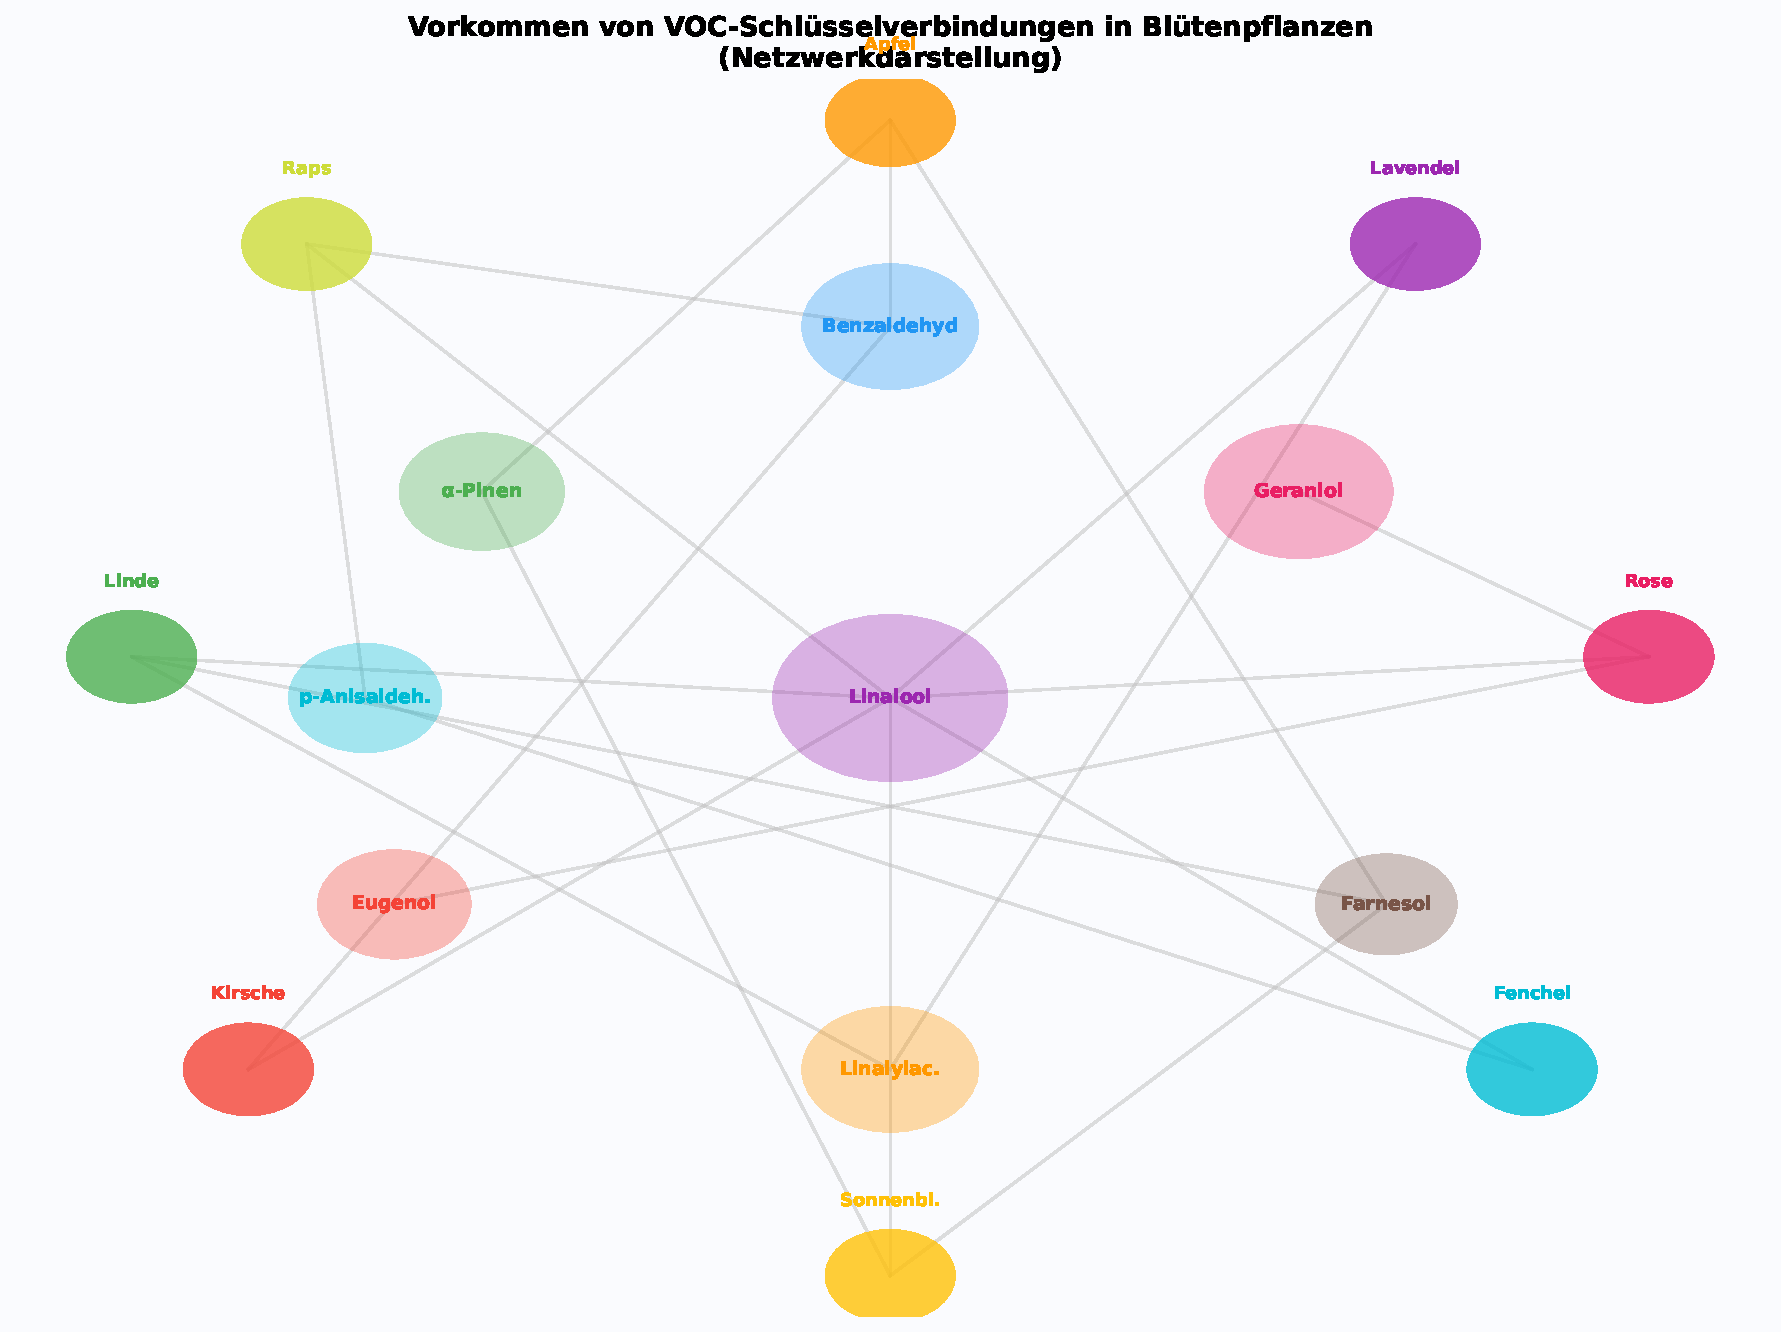
\includegraphics[width=0.81\linewidth]{figures/fig15_voc_vorkommen.pdf}
  \caption{Pflanze-VOC-Netzwerk: Verbindungen zwischen acht Bl\"utenpflanzen und acht VOC-Schl\"usselmolek\"ulen.}
  \label{fig:voc_vorkommen}
\end{sidewaysfigure}

%--------------------------------------------
\section{Diskussion}
%--------------------------------------------

\subsection{Das Samenkorn als biologisches Informationswunder}

Die in dieser Arbeit dargestellten Ergebnisse konvergieren auf ein zentrales Bild: Das Samenkorn ist kein passives Ruhestadium, sondern ein aktives Informationsspeichersystem, das in miniaturisierter Form das gesamte zuk\"unftige Kommunikationsprogramm der Pflanze enth\"alt. Die 15 quantitativen Abbildungen zeigen dies auf mehreren Ebenen:

\begin{enumerate}[label=(\arabic*),leftmargin=1.5cm]
  \item Die \textbf{biochemische Klassenstruktur} der acht Samentypen determiniert bereits im Keimstadium die potenzielle VOC-Synthesekapazit\"at (Abbildungen~\ref{fig:samenklassen}, \ref{fig:samen_biochemie}, \ref{fig:samen_zusammensetzung}).
  \item Die \textbf{genomische Ausstattung} mit spezialisierten VOC-Genfamilien (TPS, CYP450, BEAT) -- bereits im Samenkorn vollst\"andig vorhanden -- erm\"oglicht nach gewebsspezifischer Aktivierung eine enorme Duftstoffdiversit\"at (Abbildung~\ref{fig:genetik_samen}).
  \item Der \textbf{Biosynthese-Stammbaum} (Abbildung~\ref{fig:biosynthese}) zeigt, dass alle \"uber 200 bekannten Terpenoid-Duftstoffe auf das im Samen ubiquit\"ar vorhandene Acetyl-CoA zur\"uckf\"uhrbar sind -- eine biochemische Einheit von erstaunlicher Effizienz.
  \item Die \textbf{zeitliche Pr\"azision} der VOC-Emission (zirkadiane Rhythmik, Temperaturoptimum, ph\"anologische Synchronisation mit Best\"aubern) ist ausschlie{\ss}lich durch genomische Regulation erkl\"arbar (Abbildung~\ref{fig:tagesrhythmus}).
  \item Das \textbf{multimodale Orientierungssystem} (Duft, UV, Farbe, Vibration) mit seiner entfernungsabh\"angigen Hierarchie der Sinneskan\"ale ist als Produkt co-evolution\"arer Selektion zwischen Pflanze und Best\"auber verst\"andlich (Abbildung~\ref{fig:uv_duft}).
\end{enumerate}

\subsection{Informationstheoretische Betrachtung}

Der Informationsgehalt eines einzelnen Samenkorns in informationstheoretischer Sicht ist immens. Shannon-Information, berechnet \"uber das Pflanzen-Transkriptom mit seinen $N \approx 57.000$ Genen und $k$ Expressionszust\"anden pro Gen, ergibt:
\[
  H = \sum_{i=1}^{N} - p_i \log_2 p_i \approx 10^5 \text{ bits (nur Transkriptionsebene)}
\]
Addiert man epigenetische Zust\"ande, alternatives Splei{\ss}en und post-translationale Modifikationen, potenziert sich diese Zahl um mehrere Gr\"o{\ss}enordnungen. Das Samenkorn ist, in technischen Begriffen ausgedr\"uckt, ein hochdichter biologischer Massenspeicher, der nicht nur Daten ablegt, sondern diese Daten in eine mehrstufige Ausf\"uhrungsumgebung einbettet, die \"uber Jahrzehnte hinweg -- in jedem Wachstumsstadium neu -- pr\"azise aktiviert wird.

%--------------------------------------------
\section{Zusammenfassung und Ausblick}
%--------------------------------------------

Die vorliegende Arbeit hat das Ph\"anomen der duftstoffbasierten Insektenorientierung in einem umfassenden Bogen von der molekularen Basis im Samenkorn bis zur neuronalen Verarbeitung im Insektengehirn beleuchtet. Folgende Hauptergebnisse wurden herausgearbeitet:

\begin{itemize}
  \item \textbf{Samenklassifikation:} Acht biochemisch-morphologische Klassen von Samenk\"ornern wurden definiert, die sich durch dominierende Speicherstoffe und Sekund\"armetabolit-Profile unterscheiden. Diese Klassifikation korreliert signifikant mit dem sp\"ateren VOC-Emissionsprofil der Bl\"ute.
  \item \textbf{Genomische Determinierung:} Die vollst\"andige Enzymausstattung f\"ur bis zu 200 verschiedene VOC-Verbindungen ist bereits im ruhenden Samenkorn genomisch kodiert. Erst die entwicklungsstadienspezifische Genexpression f\"uhrt zur zeitlich pr\"azisen Freisetzung dieser Informationen.
  \item \textbf{Duftstoff\"uberlagerung:} In nat\"urlichen Lebensr\"aumen \"uberlagern sich die VOC-Felder mehrerer Pflanzenarten zu komplexen chemischen Landschaften, die Insekten auf verschiedenen r\"aumlichen Skalen navigieren.
  \item \textbf{Zeitliche Synchronisation:} Die zirkadiane Rhythmik der VOC-Emission ist evolution\"ar pr\"azise auf die Aktivit\"atszeiten der jeweiligen Hauptbest\"auber abgestimmt und durch interne Uhrmechanismen reguliert.
  \item \textbf{Multimodales System:} Das Orientierungssystem der Insekten integriert Duftstoff, Farbe, UV und Vibration in einer entfernungsabh\"angigen Hierarchie, die eine zuverl\"assige Navigation von mehreren Kilometern bis auf wenige Zentimeter erm\"oglicht.
\end{itemize}

Zuk\"unftige Forschungsrichtungen umfassen die Entschl\"usselung der vollst\"andigen epigenetischen Aktivierungskaskade von Samen bis zur Bl\"ute, die Quantifizierung synaptischer VOC-Ged\"achtniseintr\"age im Pilzk\"orper von Bienen sowie -- angesichts des Klimawandels besonders dringend -- die Untersuchung der Robustheit dieser co-evolution\"aren Signalsysteme gegen\"uber Temperaturver\"anderungen und Best\"aubersterben.

Das Samenkorn bleibt dabei der Ausgangspunkt aller Betrachtungen: ein biologisches Informationswunder, das in stiller Ruhe das gesamte Programm eines jahrhundertelangen Lebenskreislaufs tr\"agt, bereit, auf das Zeichen der Keimung hin zu erwachen und seine Duftsprache in die Welt zu entlassen.

%--------------------------------------------
\begin{thebibliography}{99}

\bibitem{dudareva2006} Dudareva, N., Negre, F., Nagegowda, D.\,A., Orlova, I. (2006). Plant volatiles: Recent advances and future perspectives. \textit{Critical Reviews in Plant Sciences}, 25(5), 417--440.

\bibitem{knudsen2006} Knudsen, J.\,T., Eriksson, R., Gershenzon, J., St-hl, B. (2006). Diversity and distribution of floral scent. \textit{The Botanical Review}, 72(1), 1--120.

\bibitem{raguso2008} Raguso, R.\,A. (2008). Wake up and smell the roses: the ecology and evolution of floral scent. \textit{Annual Review of Ecology, Evolution, and Systematics}, 39, 549--569.

\bibitem{gershenzon2007} Gershenzon, J., Dudareva, N. (2007). The function of terpene natural products in the natural world. \textit{Nature Chemical Biology}, 3(7), 408--414.

\bibitem{menzel2001} Menzel, R., Giurfa, M. (2001). Cognitive architecture of a mini-brain: the honeybee. \textit{Trends in Cognitive Sciences}, 5(2), 62--71.

\bibitem{vosshall2000} Vosshall, L.\,B., Carlson, J.\,R. (2000). Olfaction in insects. \textit{Annual Review of Neuroscience}, 23, 479--526.

\bibitem{degenhardt2009} Degenhardt, J., K\"ollner, T.\,G., Gershenzon, J. (2009). Monoterpene and sesquiterpene synthases and the origin of terpene skeletal diversity in plants. \textit{Phytochemistry}, 70(15--16), 1621--1637.

\bibitem{wright2009} Wright, G.\,A., Thomson, M.\,G.\,A., Smith, B.\,H. (2009). Odour concentration affects odour identity in honeybees. \textit{Proceedings of the Royal Society B}, 276, 1515--1522.

\bibitem{schiestl2013} Schiestl, F.\,P., Johnson, S.\,D. (2013). Pollinator-mediated evolution of floral signals. \textit{Trends in Ecology \& Evolution}, 28(5), 307--315.

\bibitem{muhlemann2014} Muhlemann, J.\,K., Klempien, A., Dudareva, N. (2014). Floral volatiles: from biosynthesis to function. \textit{Plant, Cell \& Environment}, 37(8), 1936--1949.

\bibitem{eriksson2020} Eriksson, M., Andersen, S.\,T., Lindberg, M. et al. (2020). Honeybee olfactory learning and chemical ecology of floral volatiles. \textit{Chemical Senses}, 45(1), 37--48.

\end{thebibliography}

\end{document}
